% !TEX program = xelatex

\documentclass[16pt,a4]{internshipreport}

\usepackage{lipsum}  
\usepackage[numbib]{tocbibind}
\usepackage{appendix}
\usepackage{float}
\usepackage{wrapfig}

\title{การเขียนรายงานฝึกงานที่เขียนเทมเพลทนานกว่ารายงาน}
\entitle{Writing a nonsensible internship report just to test the template}
\location{ครัวป้าวง ป่ายุบใน}
\date{2562}
\author{ศิระกร ลำใย}
\studentid{5910500023}

\begin{document}

\maketitle

\chapter*{บทคัดย่อ}
\addcontentsline{toc}{chapter}{บทคัดย่อ}
\lipsum[2-4]

\chapter*{กิตติกรรมประกาศ}
\addcontentsline{toc}{chapter}{กิตติกรรมประกาศ}
ประการแรก ข้าพเจ้าขอขอบพระคุณครอบครัวที่สนับสนุนและตัดสินใจให้ทำในสิ่งที่เชื่อว่าถูกต้องมาโดยตลอด
การให้อิสระทางความคิดและการตัดสินใจนั้นเป็นสิ่งที่จำเป็น มีค่าอย่างยิ่ง และสร้างเสริมประสบการณ์ที่แข็งแรง
ในการตัดสินใจทำหลายๆ อย่าง

ขอขอบพระคุณอาจารย์ธีรวิทย์ วิไลประสิทธิ์พร จากสถาบันวิทยสิริเมธี และอาจารย์ธนาวินท์ รักธรรมานนท์
จากมหาวิทยาลัยเกษตรศาสตร์ สำหรับการสนับสนุนในการฝึกงานทั้งในช่วงปี 2561 และปี 2562 (กล่าวคือในสองปีที่ผ่านมา)

ขอขอบพระคุณอาจารย์จากภาควิชาวิศวกรรมคอมพิวเตอร์ และวิศวกรรมไฟฟ้า มหาวิทยาลัยเกษตรศาสตร์
ผู้อยู่เบื้องหลังทัศนะคติบวก ผู้ขัดเกลามุมมองต่อโลกใบนี้ และมอบองค์ความรู้จำนวนมาก: อาจารย์จิตร์ทัศน์ ฝักเจริญผล,
อาจารย์ชัยพร ใจแก้ว, อาจารย์ธนาวินท์ รักธรรมานนท์, อาจารย์ภารุจ รัตนวนพันธุ์, อาจารย์จเร เลิศสุดวิชัย,
อาจารย์กาญจนพันธุ์ สุขวิชชัย และอื่นๆ ที่มิอาจเอ่ยนามได้หมด

ขอบคุณเป็นอย่างยิ่งในไมตรีจิตจากนิสิตและเจ้าหน้าที่ที่สถาบันวิทยสิริเมธี ผู้ซึ่งเป็นทั้งรุ่นพี่และผู้ร่วมงานที่น่ารัก: สมบัติ เกตุรัตน์
กฤษณี คำทวี, นรินทร์ คุณาเศรษฐ, ณกรณ์ ขำชัยสีเมฆ, ภุชงค์ สร้อยสุดารัตน์, (พี่ก้อง), (พี่คนอื่น)\dots

ขอขอบคุณ (หรือหากกล่าวด้วยสำนวนของข้าพเจ้า, กราบ) เพื่อนนิสิตมหาวิทยาลัยเกษตรศาสตร์ ทั้งที่ให้กำลังใจในวันที่ท้อถอย
กดดันให้พัฒนาตนเอง และมอบความมุ่งมั่นอันเต็มเปี่ยมให้: รวิสรา รัตนวรรณนุกุล, กรวิชญ์ ชัยกังวาฬ,
กิตติยา กู้เกียรติกูล, ณัฐณิชา ช้างจันทร์, วรชัย วุฒิวรชัยรุ่ง, สิรภพ กางกั้น, พรมนัส หอมเกสร,
ณัฐพงศ์ สมบูรณ์ภัทรกิจ, ปิยวัช ภวะจันทร์สถิตย์, ณัฐพล เวชกิจวาณิชย์, คุณานนต์ บุรเทพ, ณิชา ลิ้มมณี
และทุกท่านที่มิอาจเอ่ยนามได้หมด (อีกครั้ง)

ขอบคุณสมาชิก (ผู้ป้วนเปี้ยนในห้อง) กลุ่มวิจัยเชิงทฤษฎีสำหรับบรรยากาศที่สนุกยิ่งในการพักผ่อน:
ณัฐวุฒิ เพ็ชรมาก, นนทพัทธ์ วงศ์วัฒนากิจ, พงศกร อัจฉริยศักดิ์ชัย, ชยุตพงศ์ พรมภักดิ์, มณฑล จรัสตระกูล,
ภิญญพร เอี่ยมมงคล, ชวิน เอี่ยมวรวุฒิกุล, (พี่แหมง), (พี่บลู) และที่ไม่กล่าวถึงมิได้
คืออาจารย์จิตร์ทัศน์ ฝักเจริญผล อาจารย์หัวหน้ากลุ่มวิจัย

ขอบคุณวงดนตรีทุกแห่งและสมาชิกวงดนตรีทุกท่านที่ช่วยขับเคลื่อนสุนทรียศาสตร์ในการทำงาน:
วงดุริยางค์ฟิลฮาร์โมนิกแห่งประเทศไทย, วงดุริยางค์ซิมโฟนีแห่งลอนดอน, เบอร์ลินฟิลฮาร์โมนิก,
บีเอ็นเคโฟร์ตี้เอท (โดยเฉพาะสมาชิก: เฌอปราง อารีย์กุล, จิรดาภา อินทจักร, แพรวา สุธรรมพงษ์,
เจนนิษฐ์ โอ่ประเสริฐ และมณิภา รู้ปัญญา), ฟีเวอร์ (โดยเฉพาะสมาชิก: กมลพร โกสียรักษ์วงศ์,
จิรัชญา จันทร์จิเรศรัศมี, ปาลีรัตน์ ก้อนบาง, นภัสพร ศรีประภา และรัทยา ผลเกิด), ไปส่งกูบขส.ดู๊,
ชาบลูส์, นายิกา ศรีเนียน, และศิลปินจำนวนมากที่ข้าพเจ้าเสพงาน ผู้ที่มิได้เอ่ยนามมาในที่นี้

การเกิดขึ้นของสถาบันวิทยสิริเมธีจะเป็นไปไม่ได้ หากไม่ได้รับการสนับสนุนจากบริษัทปตท. จำกัด (มหาชน)
พร้อมบริษัทในเครือ และธนาคารไทยพาณิชย์ จำกัด (มหาชน) 
ข้าพเจ้าขอขอบพระคุณในความมุ่งมั่นที่จะเห็นการขับเคลื่อนนโยบายทางวิทยาศาสตร์ของประเทศจากทั้งสองบริษัท
และหวังเป็นอย่างยิ่งว่าการเกิดขี้นของสถาบันฯ จะเป็นแรงสำคัญในการผลักดันประเทศต่อไป

\tableofcontents

\listoffigures

\listoftables

\chapter{บทนำ}

\section{ความสำคัญและที่มา}
หลักสูตรวิศวกรรมศาสตรบัณฑิต สาขาวิชาวิศวกรรมคอมพิวเตอร์ หลักสูตรปรับปรุง พ.ศ 2556
ระบุให้ผู้เรียนทุกคนต้องเข้ารับการฝึกงาน เพื่อเพิ่มพูนประสบการณ์ในการเรียนรู้ที่ไม่อาจหาได้ในห้องเรียน
และเป็นการฝึกทักษะของวิศวกรในการทำงานจริง

คณะวิศวกรรมคอมพิวเตอร์ และภาควิชาวิศวกรรมคอมพิวเตอร์ จึงกำหนดให้มีการเรียนการสอนในรายวิชา
01204399 หรือการฝึกงาน แบ่งเป็นการฝึกงานภาคฤดูร้อนสำหรับนิสิตที่ไม่ได้สหกิจ
และฝึกงานต่อเนื่องในช่วงเวลาของภาคฤดูร้อนและภาคการศึกษาต้นของมหาวิทยาลัยสำหรับนิสิตที่สหกิจ
จึงเป็นที่มาของรายงานเล่มนี้ซึ่งเป็นหนึ่งในข้อกำหนด/ข้อบังคับของการฝึกงาน

\section{วัตถุประสงค์การปฏิบัติงาน}
\begin{itemize}
    \item เพื่อเพิ่มพูนประสบการณ์ในการเรียนรู้ที่ไม่อาจหาได้ในห้องเรียน
    \item เพื่อพัฒนาทักษะการทำงาน การสื่อสาร และทักษะ soft skills อื่นๆ
    \item เพื่อเป็นการเตรียมตัวในการทำโครงงานวิศวกรรมคอมพิวเตอร์ และเป็นการเตรียมตัวเขียนวารสารทางวิชาการ
\end{itemize}

\section{ขอบเขต}
ไว้มาเขียน

\section{ประวัติและรายละเอียดสถานประกอบการ}

\begin{figure}[H]
    \centering
    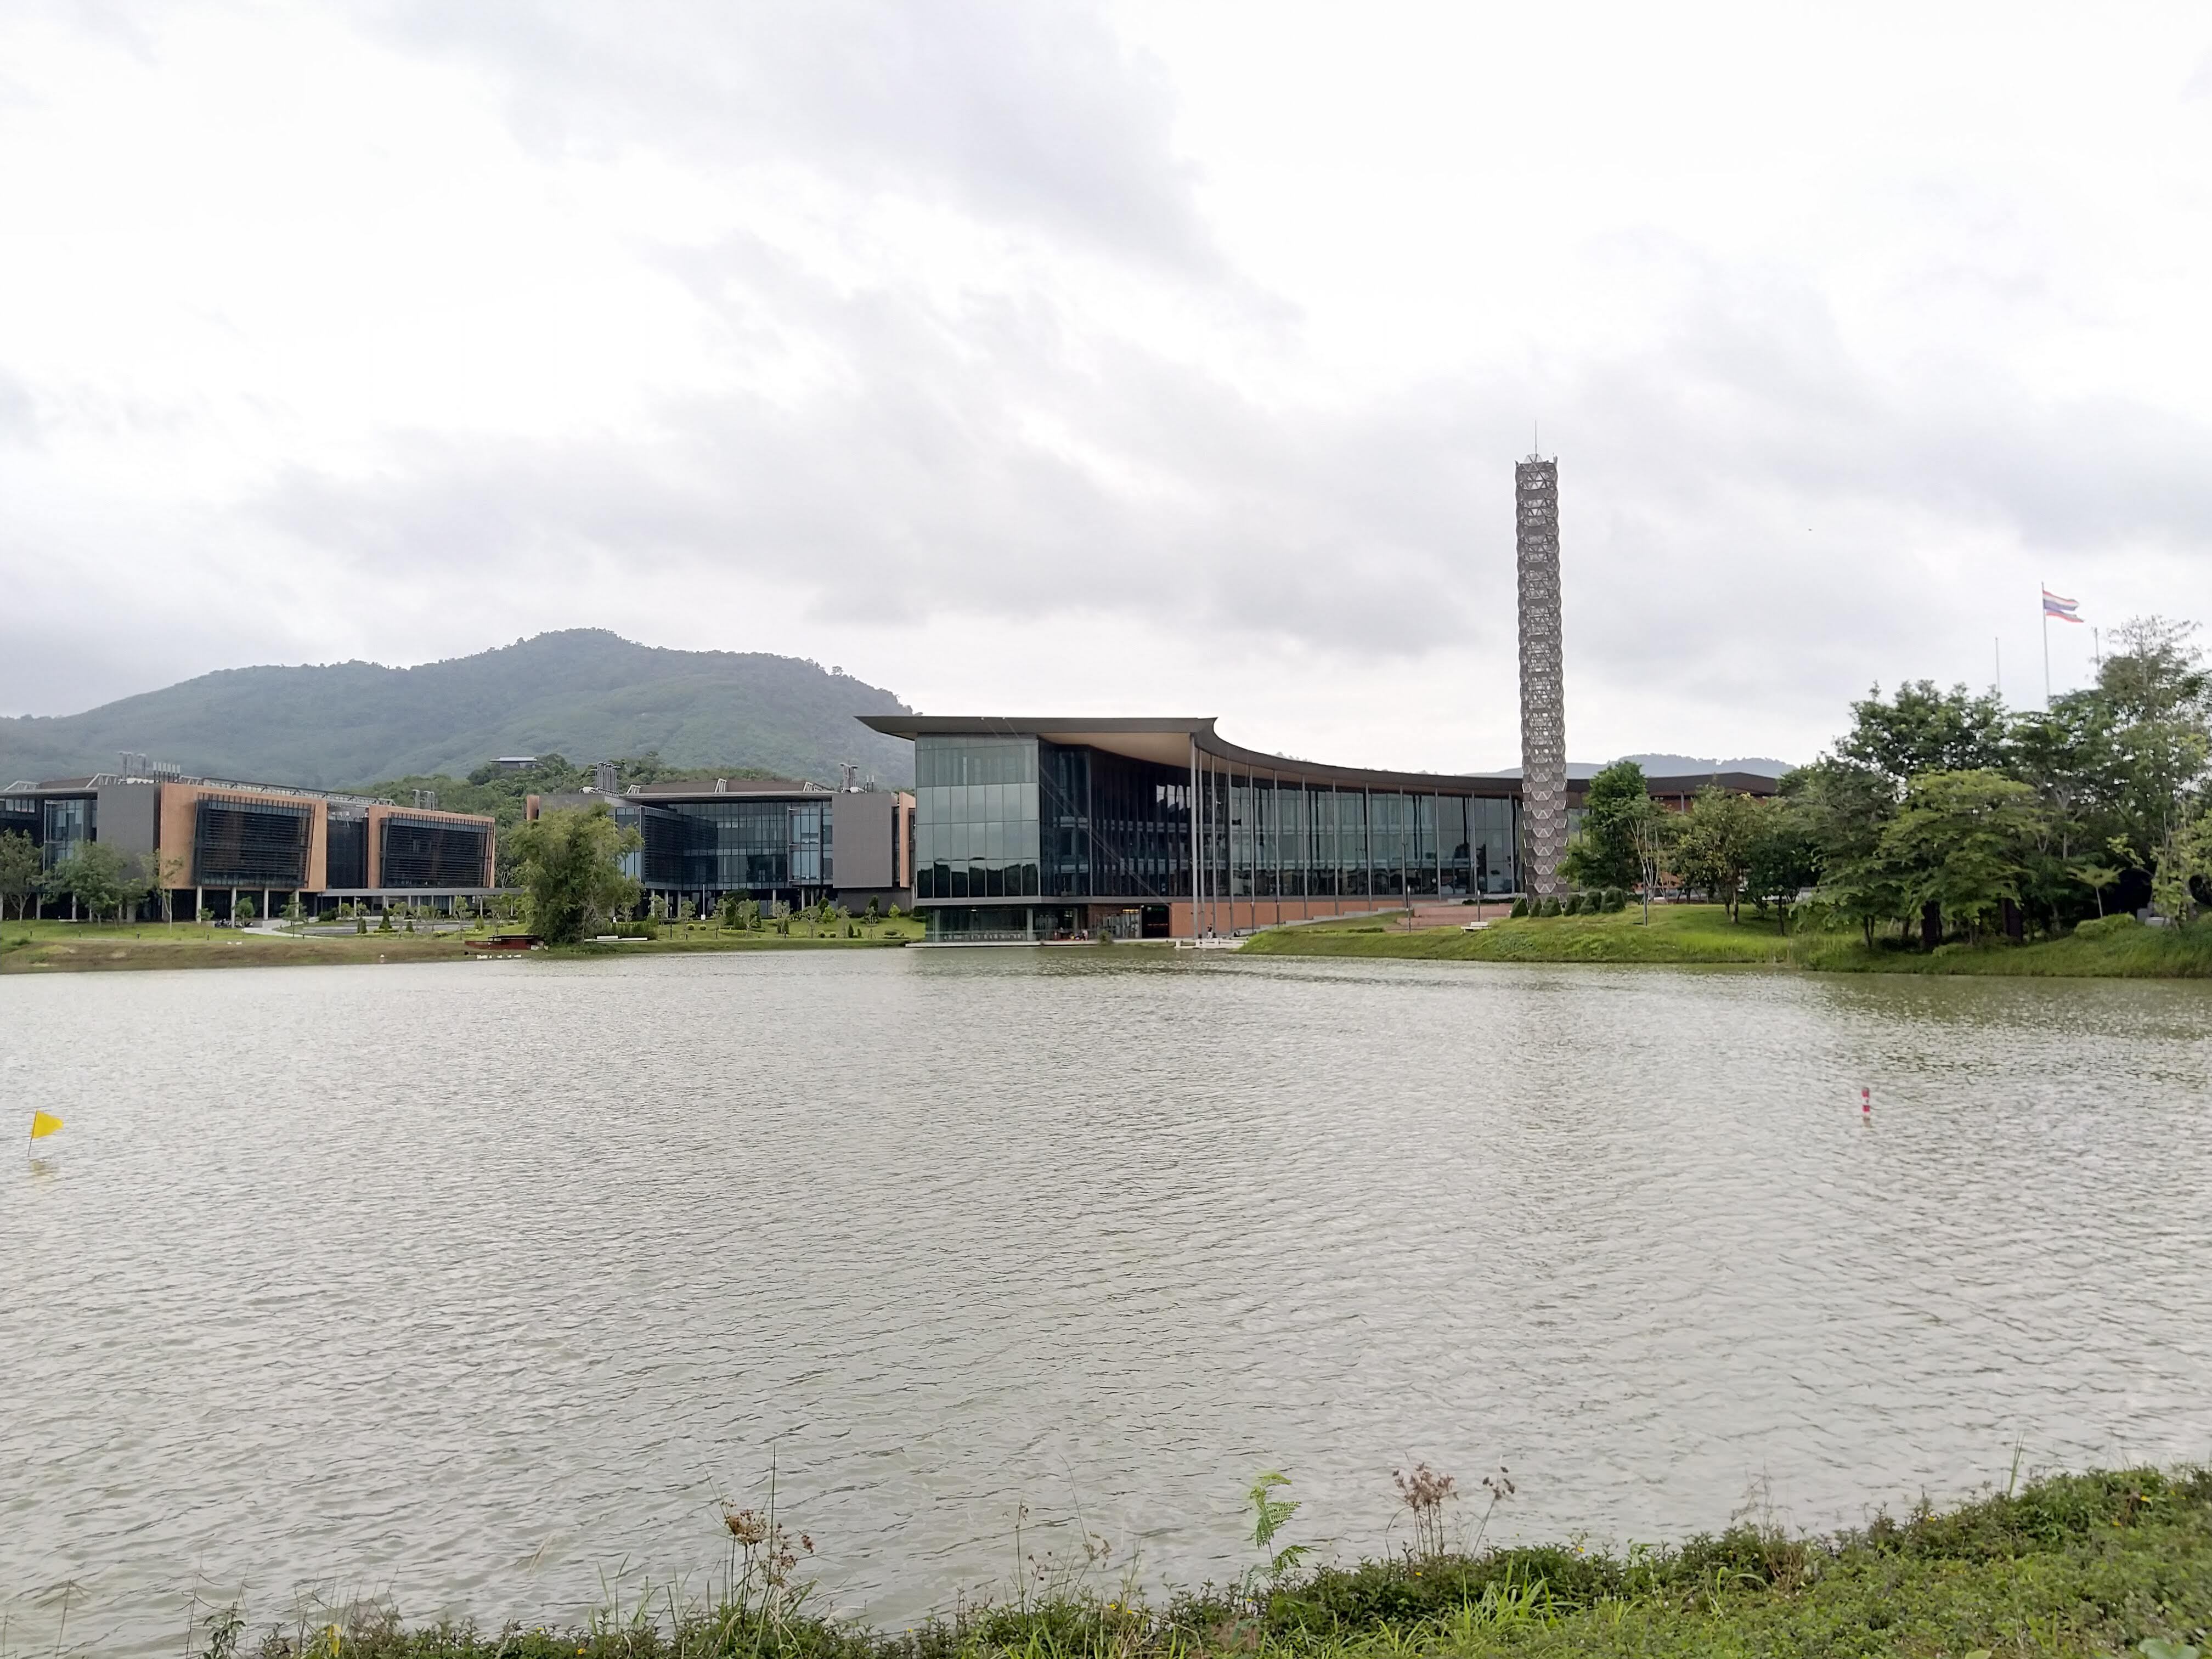
\includegraphics[width=0.8\textwidth]{images/vistec_v.jpg}
    \caption{อาคารหอสมุด สถาบันวิทยสิริเมธี}
\end{figure}

\textbf{สถาบันวิทยสิริเมธี (VISTEC)} เป็นบัณฑิตวิทยาลัย (graduate school) ซึ่งมุ่งเน้นความเป็นเลิศในการทำวิจัย 
ตั้งอยู่ในพื้นที่วังจันทร์วัลเลย์ (Wangchan Valley) และเขตนวัตกรรมระเบียงเศรษฐกิจพิเศษภาคตะวันออก
(Eastern Economic Corridor of Innovation: EECi) เลขที่ 555 หมู่ 1 ตำบลป่ายุบใน อำเภอวังจันทร์ จังหวัดระยอง
ก่อตั้งขึ้นเมื่อปี พ.ศ. 2558 โดยมูลนิธิพลังสร้างสรรค์นวัตกรรม ภายใต้การสนับสนุนเงินทุนจากบริษัท
ในกลุ่มของการปิโตรเลียมแห่งประเทศไทย (ปตท.)

VISTEC มุ่งเน้นการจัดการศึกษาด้านวิทยาศาสตร์ วิศวกรรม และเทคโนโลยี โดยมีศูนย์วิจัยวิทยาศาสตร์และเทคโนโลยีชั้นแนวหน้า
(Frontier Research Center) ซึ่งเป็นศูนย์กลาง ในการเสริมสร้างความเข้มแข็งทางการวิจัย
และให้การสนับสนุนด้านทุนการวิจัยแก่สถาบันฯ เป็นศูนย์รวมนักวิจัยที่มีความเชี่ยวชาญสูง ช่วยขับเคลื่อนการดำเนินงานด้านการศึกษา 
ิจัย การสร้างนวัตกรรม สร้างความร่วมมือทางด้านวิจัยกับสถาบันการศึกษา ภาคธุรกิจ ภาคอุตสาหกรรม
และหน่วยงานด้านการวิจัยวิทยาศาสตร์และเทคโนโลยี

\begin{figure}[H]
    \centering
    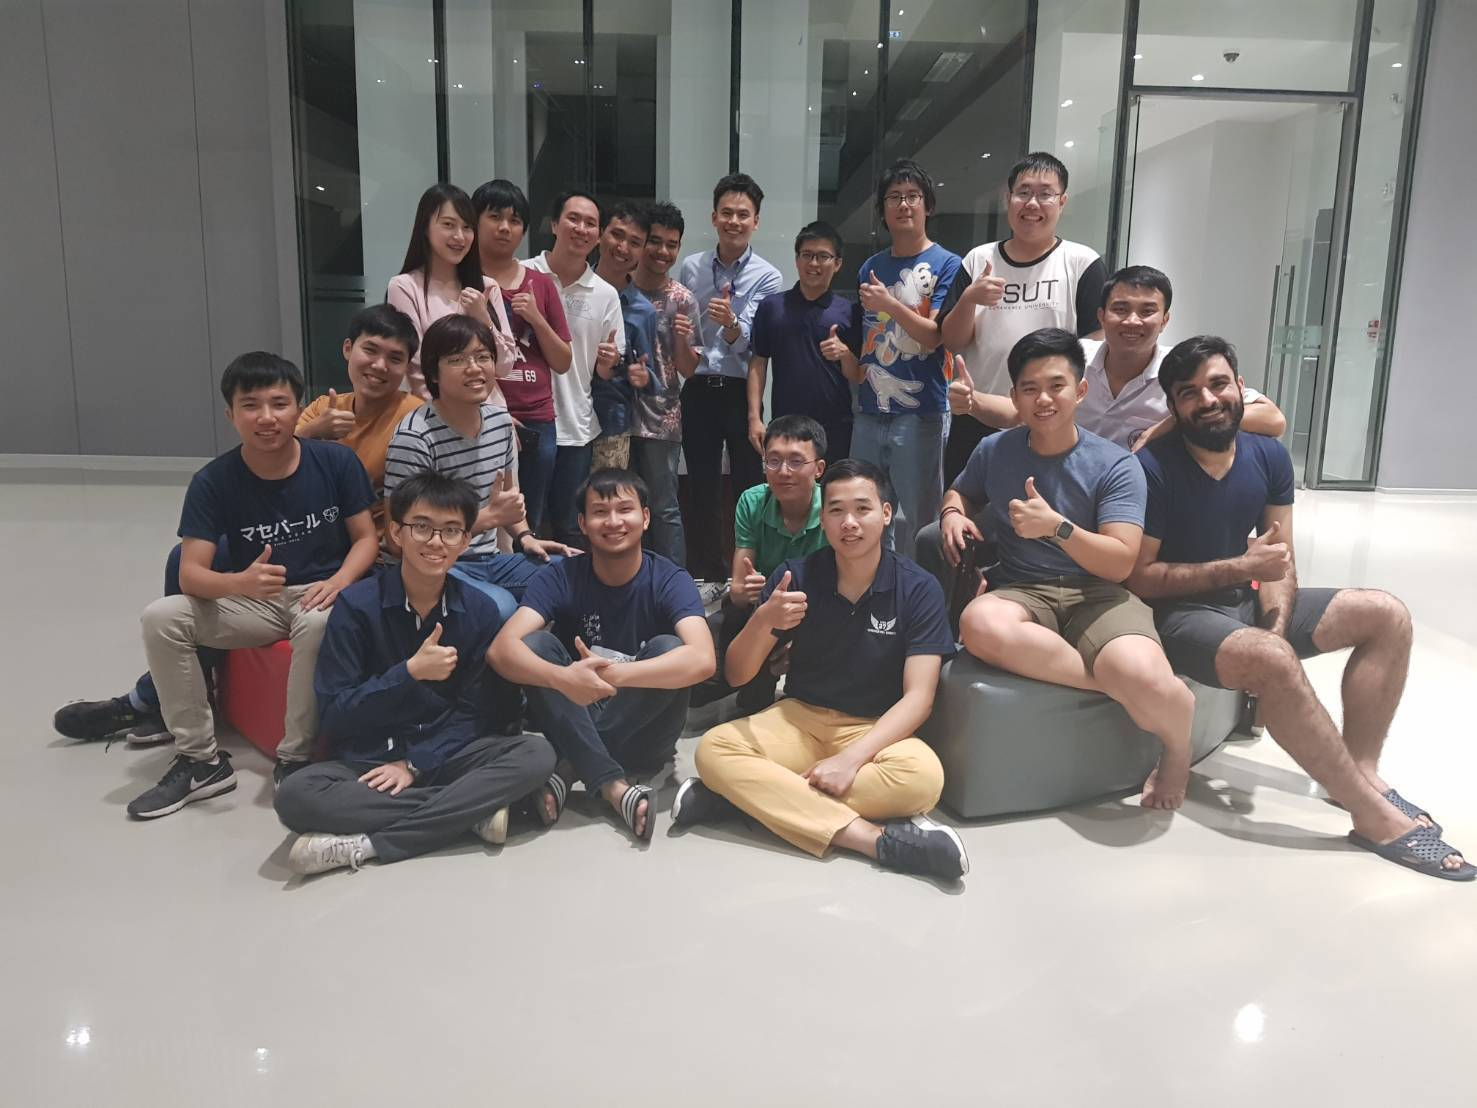
\includegraphics[width=0.8\textwidth]{images/brain_team_2018.jpg}
    \caption{ทีมวิจัย ณ ห้องปฏิบัติการ BRAIN}
\end{figure}

\textbf{ห้องปฏิบัติการเบรน (Bio-inspired Robotics and Neural Engineering: BRAIN)}
ณ สำนักวิชาวิทยาศาสตร์และเทคโนโลยีสารสนเทศ สถาบันวิทยสิริเมธี มุ่งเน้นศึกษาการสร้างหุ่นยนต์ที่มีลักษณะร่วมกับกายวิภาค
(anatomy) ของสิ่งมีชีวิต และใช้เทคโนโลยีจำพวก Machine Learning หรือ Deep Learning ในการจำแนก วิเคราะห์
และประมวลผลคลื่นสมองของมนุษย์ เพื่อสร้างส่วนติดต่อผู้ใช้ผ่านสมอง (Brain Controlled Interfaces: BCIs)

ลักษณะงานที่ได้รับผิดชอบจากห้องปฏิบัติการฯ เป็นงานของผู้ช่วยนักวิจัย (Research Assistant: RA) ซึ่งช่วยนิสิตระดับ
บัณฑิตศึกษาในการเตรียมการทดลอง ออกแบบ และพัฒนาเครื่องมือวัดผล ควบคุมการทดลอง และทดสอบสมมติฐานเพื่อตีพิมพ์
องค์ความรู้ในวารสารวิชาการต่อไป

ที่ปรึกษาและผู้ควบคุมการฝึกงานในครั้งนี้ คืออ. ดร. ธีรวิทย์ วิไลประสิทธิ์พร หัวหน้าหน่วยวิจัย (Principal Investigator: PI)
และมีระยะเวลาปฏิบัติงานประมาณ 2 เดือน กล่าวคือตั้งแต่วันที่ 4 มิถุนายน ถึง 31 กรกฎาคม 2562

\section{ประโยชน์ที่คาดว่าจะได้รับ}
เป็นการสร้างพื้นฐานในด้านงานวิจัย รวมถึงเตรียมพื้นฐานในการทำโครงงานวิศวกรรมคอมพิวเตอร์ โดยมีความมุ่งหวังจะต่อยอด
งานดังกล่าวเป็นงานวิจัยตีพิมพ์ต่อไป

\chapter{ความรู้พื้นฐานและการทบทวนวรรณกรรม}
\section{ตัวชี้วัดทางชีวภาพ}
ตัวชี้วัดทางชีวภาพ (biomarkers) เป็นตัวบ่งชี้ต่อสภาวะต่างๆ ที่เกิดกับร่างกาย ซึ่งรวมถึงแต่ไม่จำกัดเพียงแต่สถานะการตื่น สภาพอารมณ์
หรือสัญญาณบ่งชี้ของโรค

\section{คลื่นสัญญาณชีวภาพ}
คลื่นสัญญาณชีวภาพ (biosignals) เป็นคลื่นสัญญาณจากกระแสไฟฟ้าในร่างกาย ซึ่งสามารถตรวจวัดได้ด้วยวิธีการที่ต่างกันไป
และผลจากการตรวจวัดคลื่นแต่ละส่วนจะบ่งบอกซึ่งข้อมูลที่แตกต่างกันออกไปเช่นกัน

งานวิจัยของห้องปฏิบัติการเบรน มุ่งศึกษาคลื่นสัญญาณชีวภาพสามคลื่นดังต่อไปนี้

\subsection{Electroencephalography}
Electroencephalography หรือ EEG เป็นคลื่นที่เกิดจากการตรวจวัดกระแสไฟฟ้าของสมอง การตรวจวัดโดยมากไม่จำเป็นต้องทำการเจาะผิวหนัง
(noninvasive) โดยใช้อิเล็กโทรดนำไฟฟ้าอ่านคลื่นสมองจากกระโหลก

การตรวจวัดและใช้ข้อมูลจากคลื่น EEG ส่วนมากมุ่งเน้นการใช้ศักย์ไฟฟ้าที่ขึ้นกับเหตุการณ์กระตุ้นของผู้ถูกวัด
(Event Related Potential) กล่าวคือมุ่งสังเกตจุดสูงสุดและต่ำสุดของศักย์ไฟฟ้าของคลื่นสมอง
และหาความสัมพันธ์ระหว่างเหตุการณ์กระตุ้นและการเพิ่มขึ้นหรือลดลงของศักย์ไฟฟ้า
\begin{appendices}
\chapter{บันทึกประจำวัน}
\section*{4/6/2562}

เนื่องจากเข้าทำงานเป็นวันแรก จึงต้องจัดสถานที่ทำงาน และทำงานต่อจากที่ได้รับมอบหมายก่อนการฝึกงาน

งานที่ได้รับมอบหมายโดยคร่าวคือการวิเคราะห์สภาวะความง่วงในคน โดยศึกษาจากกลุ่มเป้าหมายของพนักงานบริษัท
ซึ่งอาจารย์ที่ปรึกษาให้สิทธิ์ในการกำหนดแนวทางการวิเคราะห์ได้โดยอิสระ อย่างไรก็ตามงานของการวิเคราะห์ความง่วง
โดยตั้งต้นนั้นมักใช้การวิเคราะห์ภาพจากดวงตา (gaze monitoring) ซึ่งใช้วันนี้ในการหางานวิจัยตั้งต้น

นอกจากนี้ยังศึกษาแนวทาง ข้อกำหนด และมาตรฐานจริยธรรมในการทดลองภายในมนุษย์ (human subject research)

\section*{5/6/2562}

ศึกษาแนวทางในการทำ eye gazing ตามหนังสือที่ได้รับมอบหมาย และนำเสนองานวิจัยต่อจากที่เลือกจากเมื่อวาน

ปรับแก้แนวทางในการวิจัย และได้รับมอบหมายให้ออกแบบวิธีการทดลองโดยคร่าว
หารือกับทีมโปรแกรมเมอร์ว่าด้วยซอฟต์แวร์สำหรับการทดลอง

\section*{6/6/2562}

ศึกษาอุปกรณ์สำหรับติดตามดวงตา (Gazepoint) ก่อนจะพบว่าอุปกรณ์มีข้อจำกัดในการทำงานบางส่วน ทำให้ไม่สามารถดึง
ภาพดวงตาออกมาใช้ในโปรแกรมภายนอกได้ และติดต่อกับผู้ผลิตอุปกรณ์เพื่อหารือความเป็นไปได้ในการดึงภาพดวงตา

ศึกษาการใช้ Pytorch ในการทำการเรียนรู้เชิงลึก (deep learning) แทนที่ Keras

\section*{7/6/2562}

เปลี่ยนแนวทางการทำวิจัยด้วยข้อจำกัดของอุปกรณ์ มาเป็นการทำวิจัยบนกล้ามเนื้อตา (EOG) ค้นคว้าและทบทวนวรรรณกรรม
ที่เกี่ยวข้องกับงาน

ทำแบบทดสอบสำหรับบทเรียนจริยธรรมการวิจัยในมนุษย์จนอยู่ในเกณฑ์ได้รับประกาศนียบัตรผ่านการอบรม

\section*{10/6/2562}

นักเรียนจากโครงการพัฒนาอัจฉริยภาพทางวิทยาศาสตร์เข้ามาร่วมในทีม โดยการทดลองในส่วนของ Drowsiness research
ถูกแบ่งออกเป็นสองงานที่ต้องทดลองร่วมกัน จึงต้องตกลงแนวทางการทดลองให้ชัดเจน

ทดลองให้นักเรียนดังกล่าวศึกษาการวัดคลื่นสมองโดยอุปกรณ์ OpenBCI, ให้คำแนะนำถึงการเตรียมผิวหนัง (skin preparation)
ก่อนการติดอิเล็กโทรด, การเลือกใช้ชนิดอิเล็กโทรดและข้อดี-ข้อเสียของอิเล็กโทรดแต่ละชนิด

\section*{11/6/2562}

ทำงานที่ได้รับมอบหมายต่อจากเมื่อวาน

\section*{12/6/2562}

นัดประชุมงานกับอาจารย์ที่ปรึกษาโครงการ สรุปแนวทางการทดลอง และตัดสินใจเพิ่มการวัด PVT (Psychomotor vigilance task)
เพิ่มเติมในการทดลอง

เขียนโปรแกรมสำหรับทดสอบ PVT โดยใช้การสื่อสารบนอุปกรณ์หลายเครื่องเพื่อลดความจำเป็นในการซื้อปุ่ม (physical button)
ด้วยเหตุผลทางงบประมาณ

ช่วงเย็นรับประทานอาหารเย็นร่วมกับอาจารย์ธงชัย ชิวปรีชา

\section*{13/6/2562}

ได้รับมอบหมายให้ทดลองจับภาพตาเพื่อหา PERCLOS ด้วยกล้องเว็บแคมแบบที่มีหลอดอินฟราเรด ในเบื้องต้นสามารถครอปตัดเฉพาะส่วน
ที่เป็นลูกตาออกจากภาพใบหน้าแบบเต็มหน้าได้ อย่างไรก็ตาม ไม่ประสบความสำเร็จในการคำนวนร้อยละพื้นที่ของตาดำที่ไม่ถูกหนังตาบดบัง

\begin{figure}[H]
    \centering
    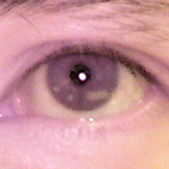
\includegraphics[width=0.4\textwidth]{images/268.png}
    \caption{ภาพถ่ายตาจากล้อง IR}
\end{figure}

\section*{14/6/2562}

ศึกษาและทบทวนวรรณกรรมว่าด้วยการประมวลผลภาพลูกตา และนำมาประยุกต์เขียนบนไลบรารี่ OpenCV จนสามารถสกัดตำแหน่งงของตาออกมา
จากภาพถ่ายของใบหน้าผู้ใช้ได้

ตัดสินใจเปลี่ยนจากเว็บแคมพร้อมหลอด IR เป็นกล้องธรรมดา

\begin{figure}[H]
    \centering
    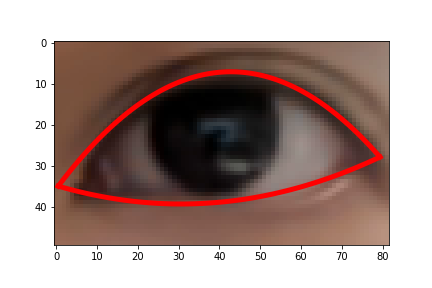
\includegraphics[width=0.4\textwidth]{images/111.png}
    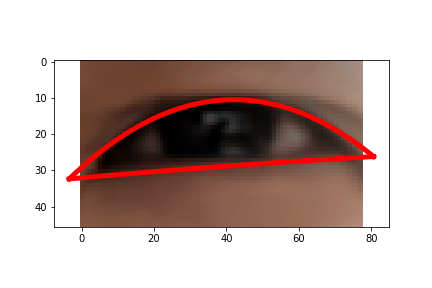
\includegraphics[width=0.4\textwidth]{images/171.png}
    \caption{ภาพถ่ายตาจากล้องที่ประมวลผลภาพเพื่อหาตำแหน่งของดวงตา ทั้งกรณีที่เปิดและปิดตา โดยประมวลผลภาพออกมาเป็นที่เรียบร้อย}
\end{figure}

\section*{17/6/2562}

ได้รับมอบหมายกระทันหันให้ร่วมเขียนเปเปอร์กับทีม SSVEP จีงเปลี่ยนสโคปงานเป็นการเขียนเปเปอร์ให้สามารถส่งตีพิมพ์ได้เร็วที่สุด

ศึกษาการใช้งานเครื่องมือทางสถิติ และทบทวนวรรณกรรมเท่าที่จำเป็น

\section*{18/6/2562}

เขียน ทบทวน และตรวจทานงานวิจัย

\section*{19/6/2562}

เขียน ทบทวน และตรวจทานงานวิจัยต่อ

\section*{20/6/2562}

เขียน ทบทวน และตรวจทานงานวิจัยต่อ

\section*{21/6/2562}

เขียน ทบทวน และตรวจทานงานวิจัยต่อ

\section*{24/6/2562}

เขียน ทบทวน และตรวจทานงานวิจัยต่อ

\section*{25/6/2562}

เขียน ทบทวน และตรวจทานงานวิจัยต่อ
\chapter{ภาพถ่ายสถานที่ปฏิบัติงาน}

\section*{ภาพการฝึกงานวันที่ 4/6/2562}
\begin{figure}[H]
    \centering
    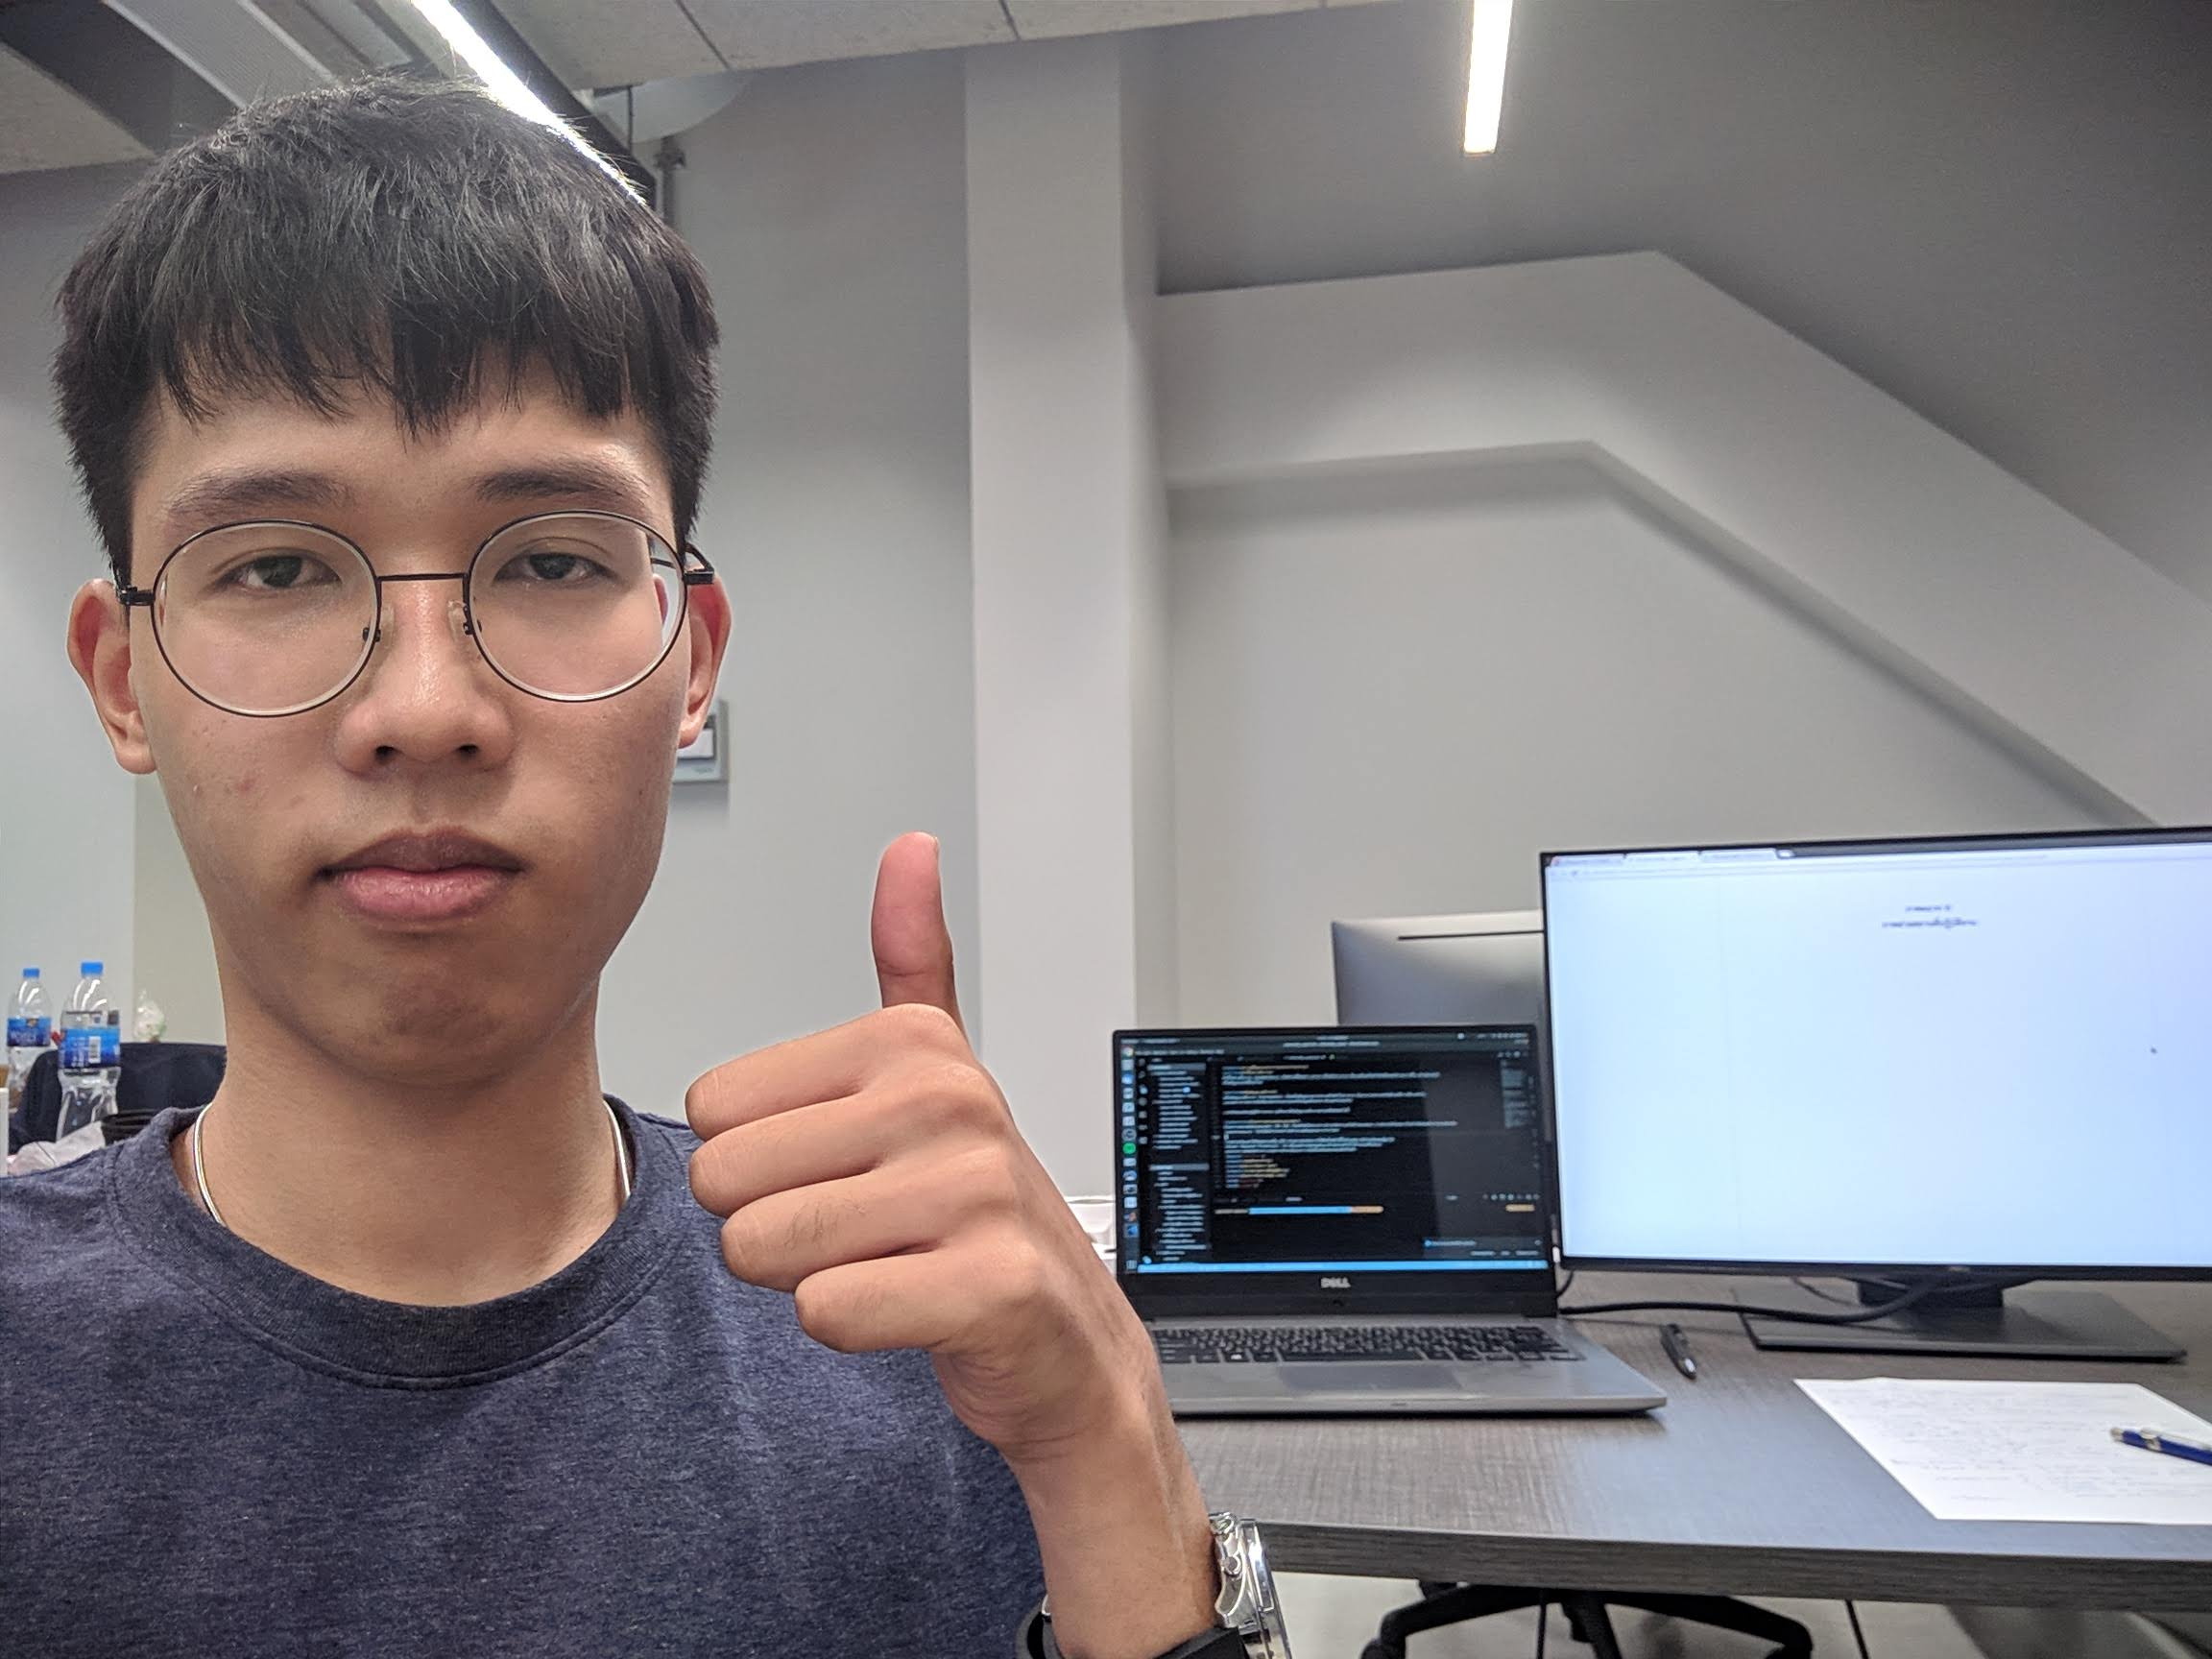
\includegraphics[width=0.55\textwidth]{/home/srakrn/Works/senior/internship/internship_report/diary/images/IMG_20190604_152401.jpg}
    \caption{สถานที่ทำงานหลังจากจัดที่ทำงานแล้ว}
\end{figure}

\section*{ภาพการฝึกงานวันที่ 5/6/2562}
\begin{figure}[H]
    \centering
    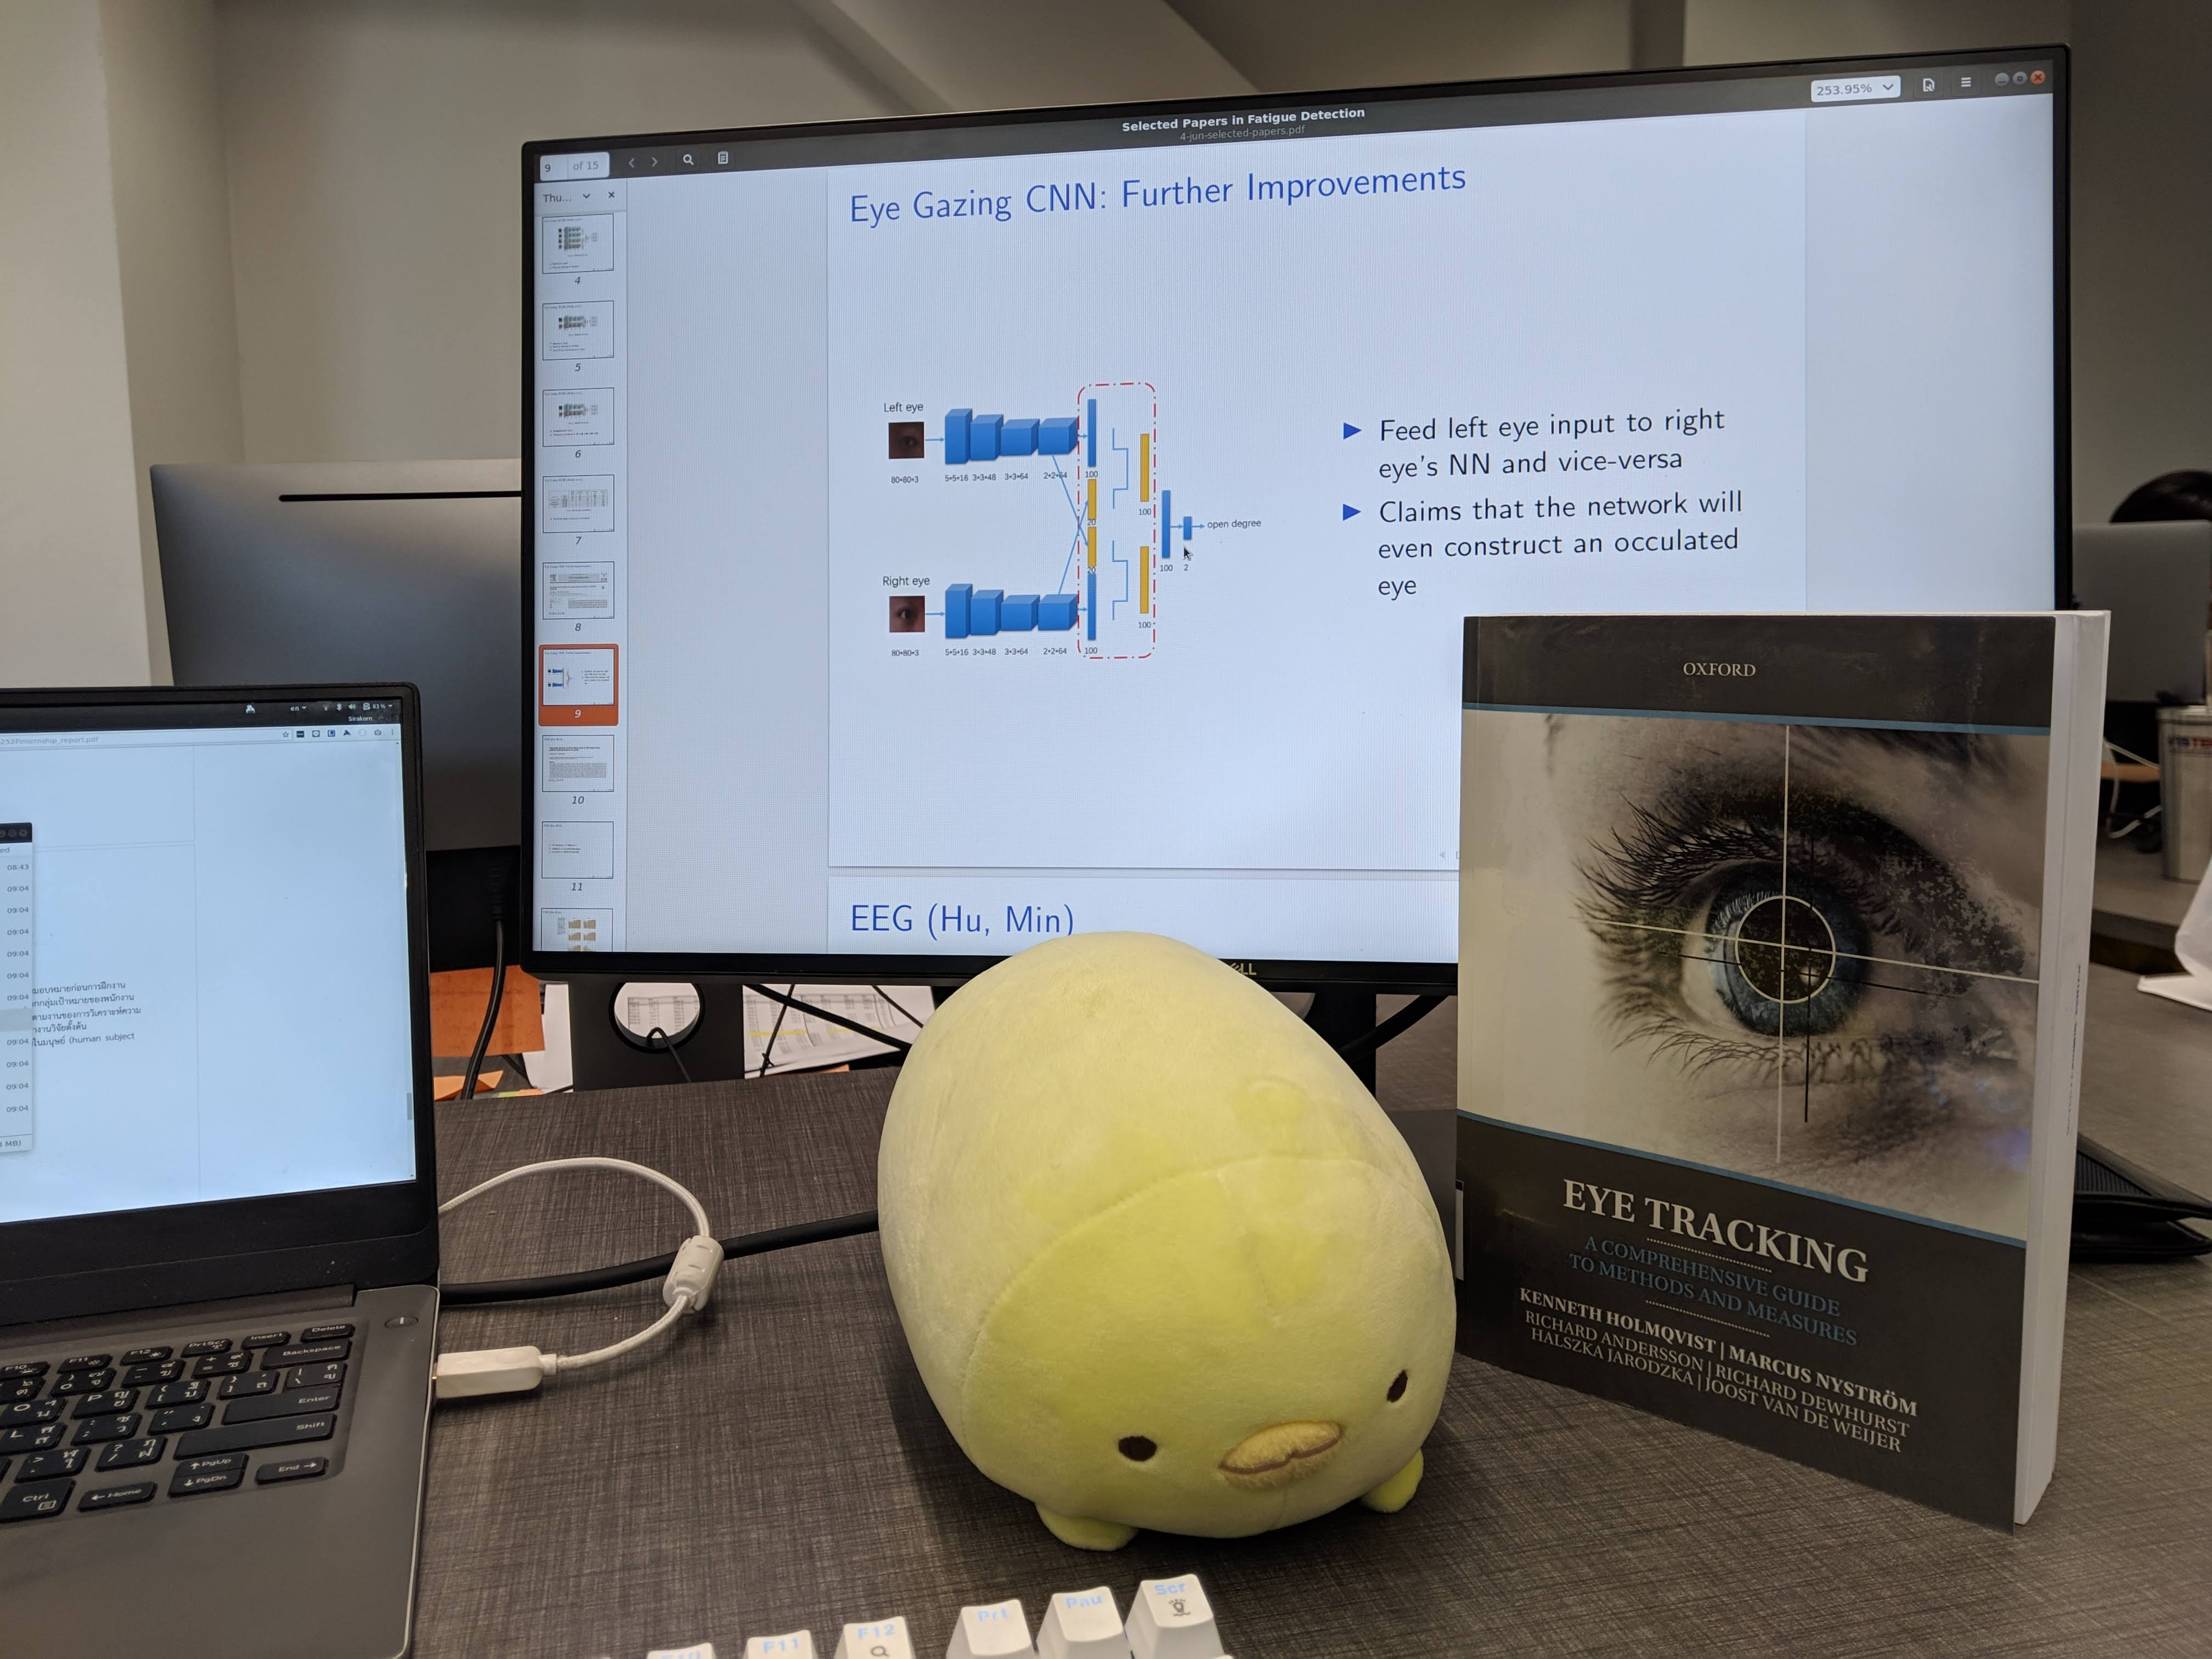
\includegraphics[width=0.55\textwidth]{/home/srakrn/Works/senior/internship/internship_report/diary/images/IMG_20190605_112217.jpg}
    \caption{หนังสือที่ได้รับมอบหมายให้อ่านและศึกษา ถ่ายคู่กับสไลด์สรุปงานวิจัย}
\end{figure}

\section*{ภาพการฝึกงานวันที่ 6/6/2562}
\begin{figure}[H]
    \centering
    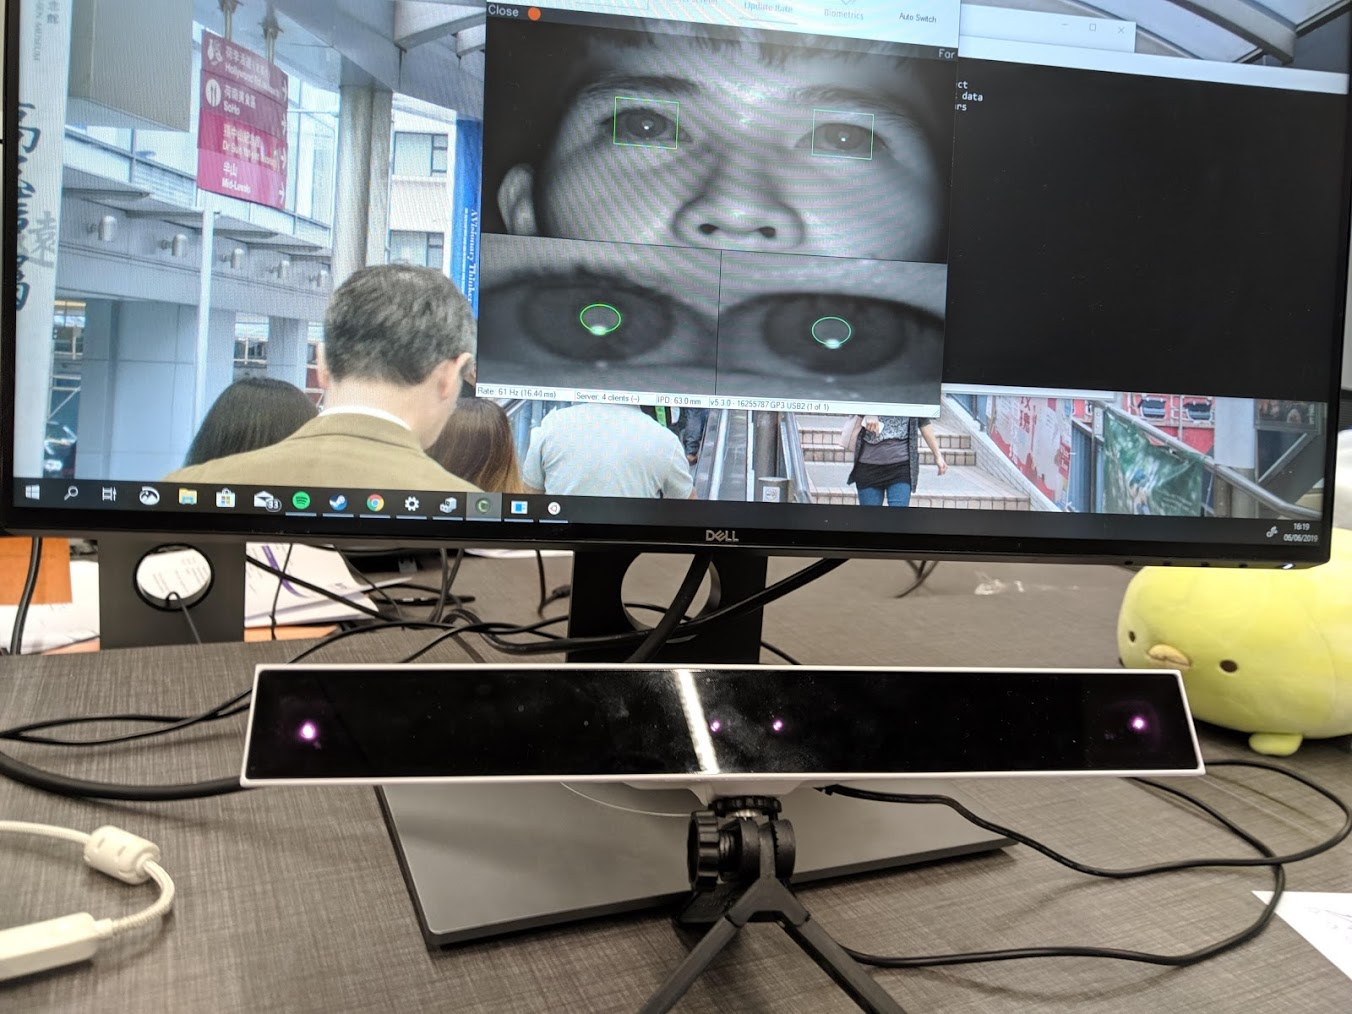
\includegraphics[width=0.55\textwidth]{/home/srakrn/Works/senior/internship/internship_report/diary/images/IMG_20190606_161925.jpg}
    \caption{อุปกรณ์สำหรับติดตามดวงตา Gazepoint ขณะกำลังจับม่านตา}
\end{figure}

\section*{ภาพการฝึกงานวันที่ 10/6/2562}
\begin{figure}[H]
    \centering
    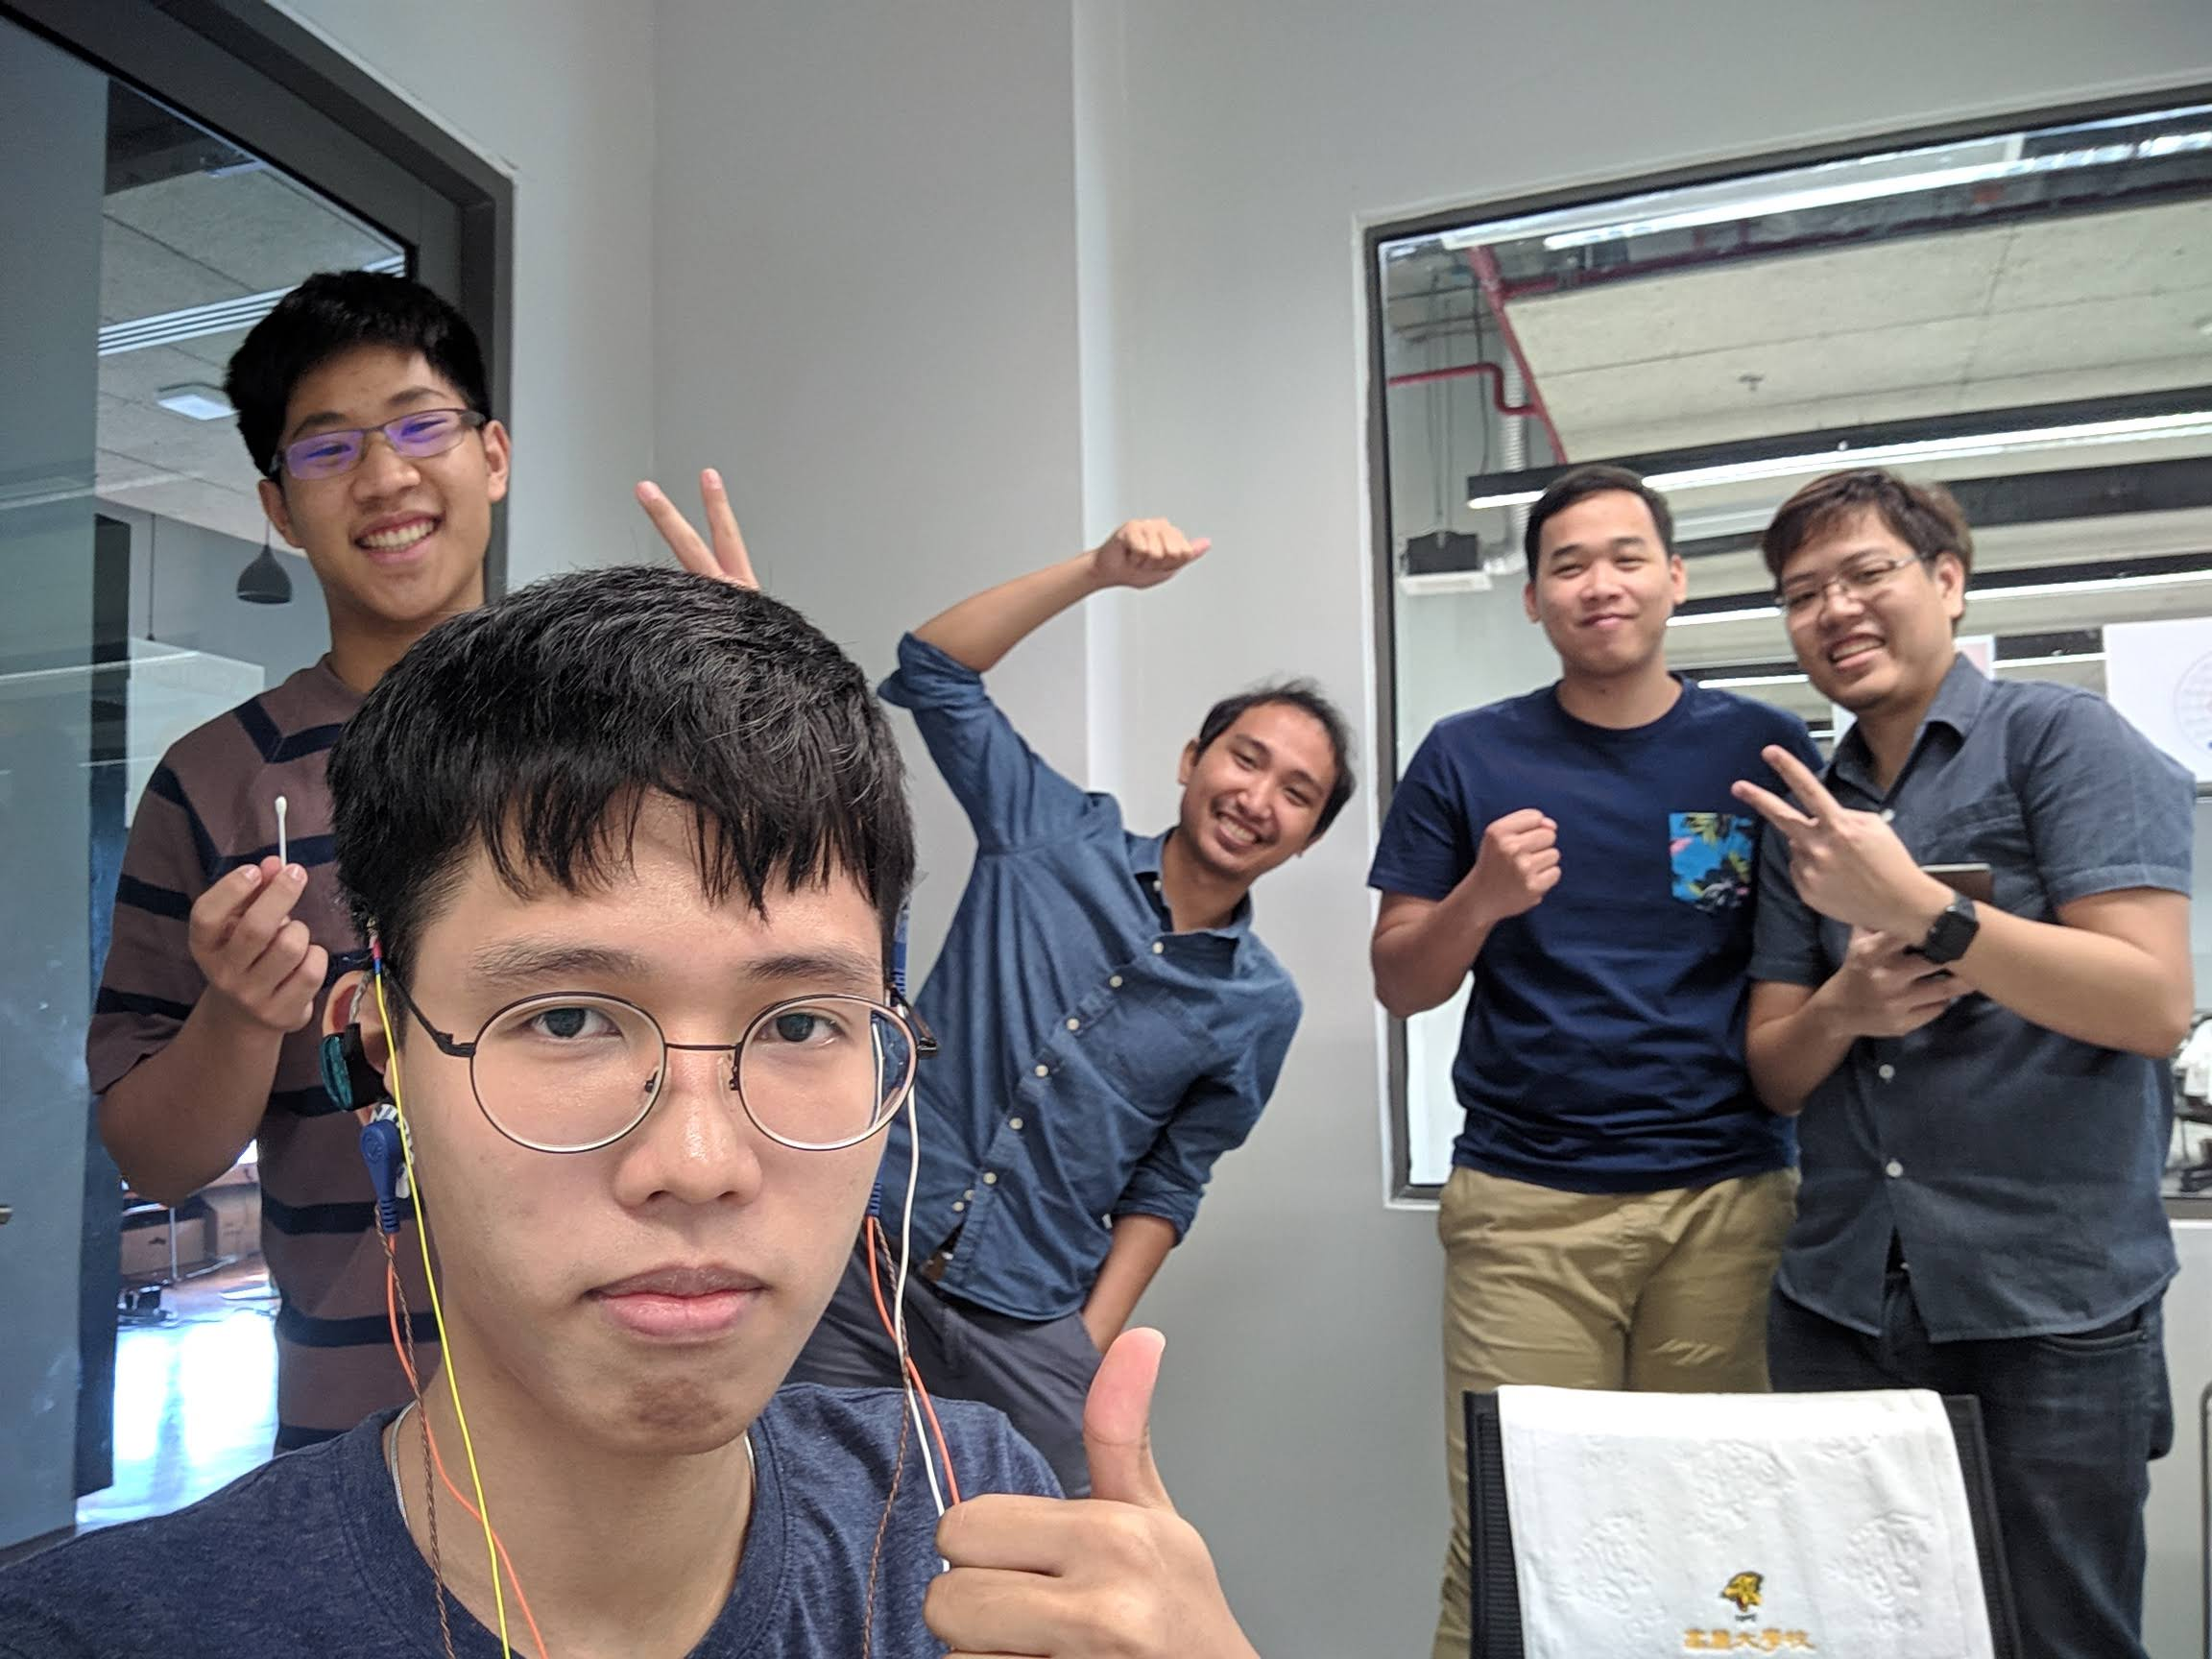
\includegraphics[width=0.55\textwidth]{/home/srakrn/Works/senior/internship/internship_report/diary/images/IMG_20190610_155035.jpg}
    \caption{สมาชิกทีม Drowsiness Research และสมาชิกทีม BRAIN ขณะทดสอบสมมติฐาน}
\end{figure}

\section*{ภาพการฝึกงานวันที่ 24/6/2562}
\begin{figure}[H]
    \centering
    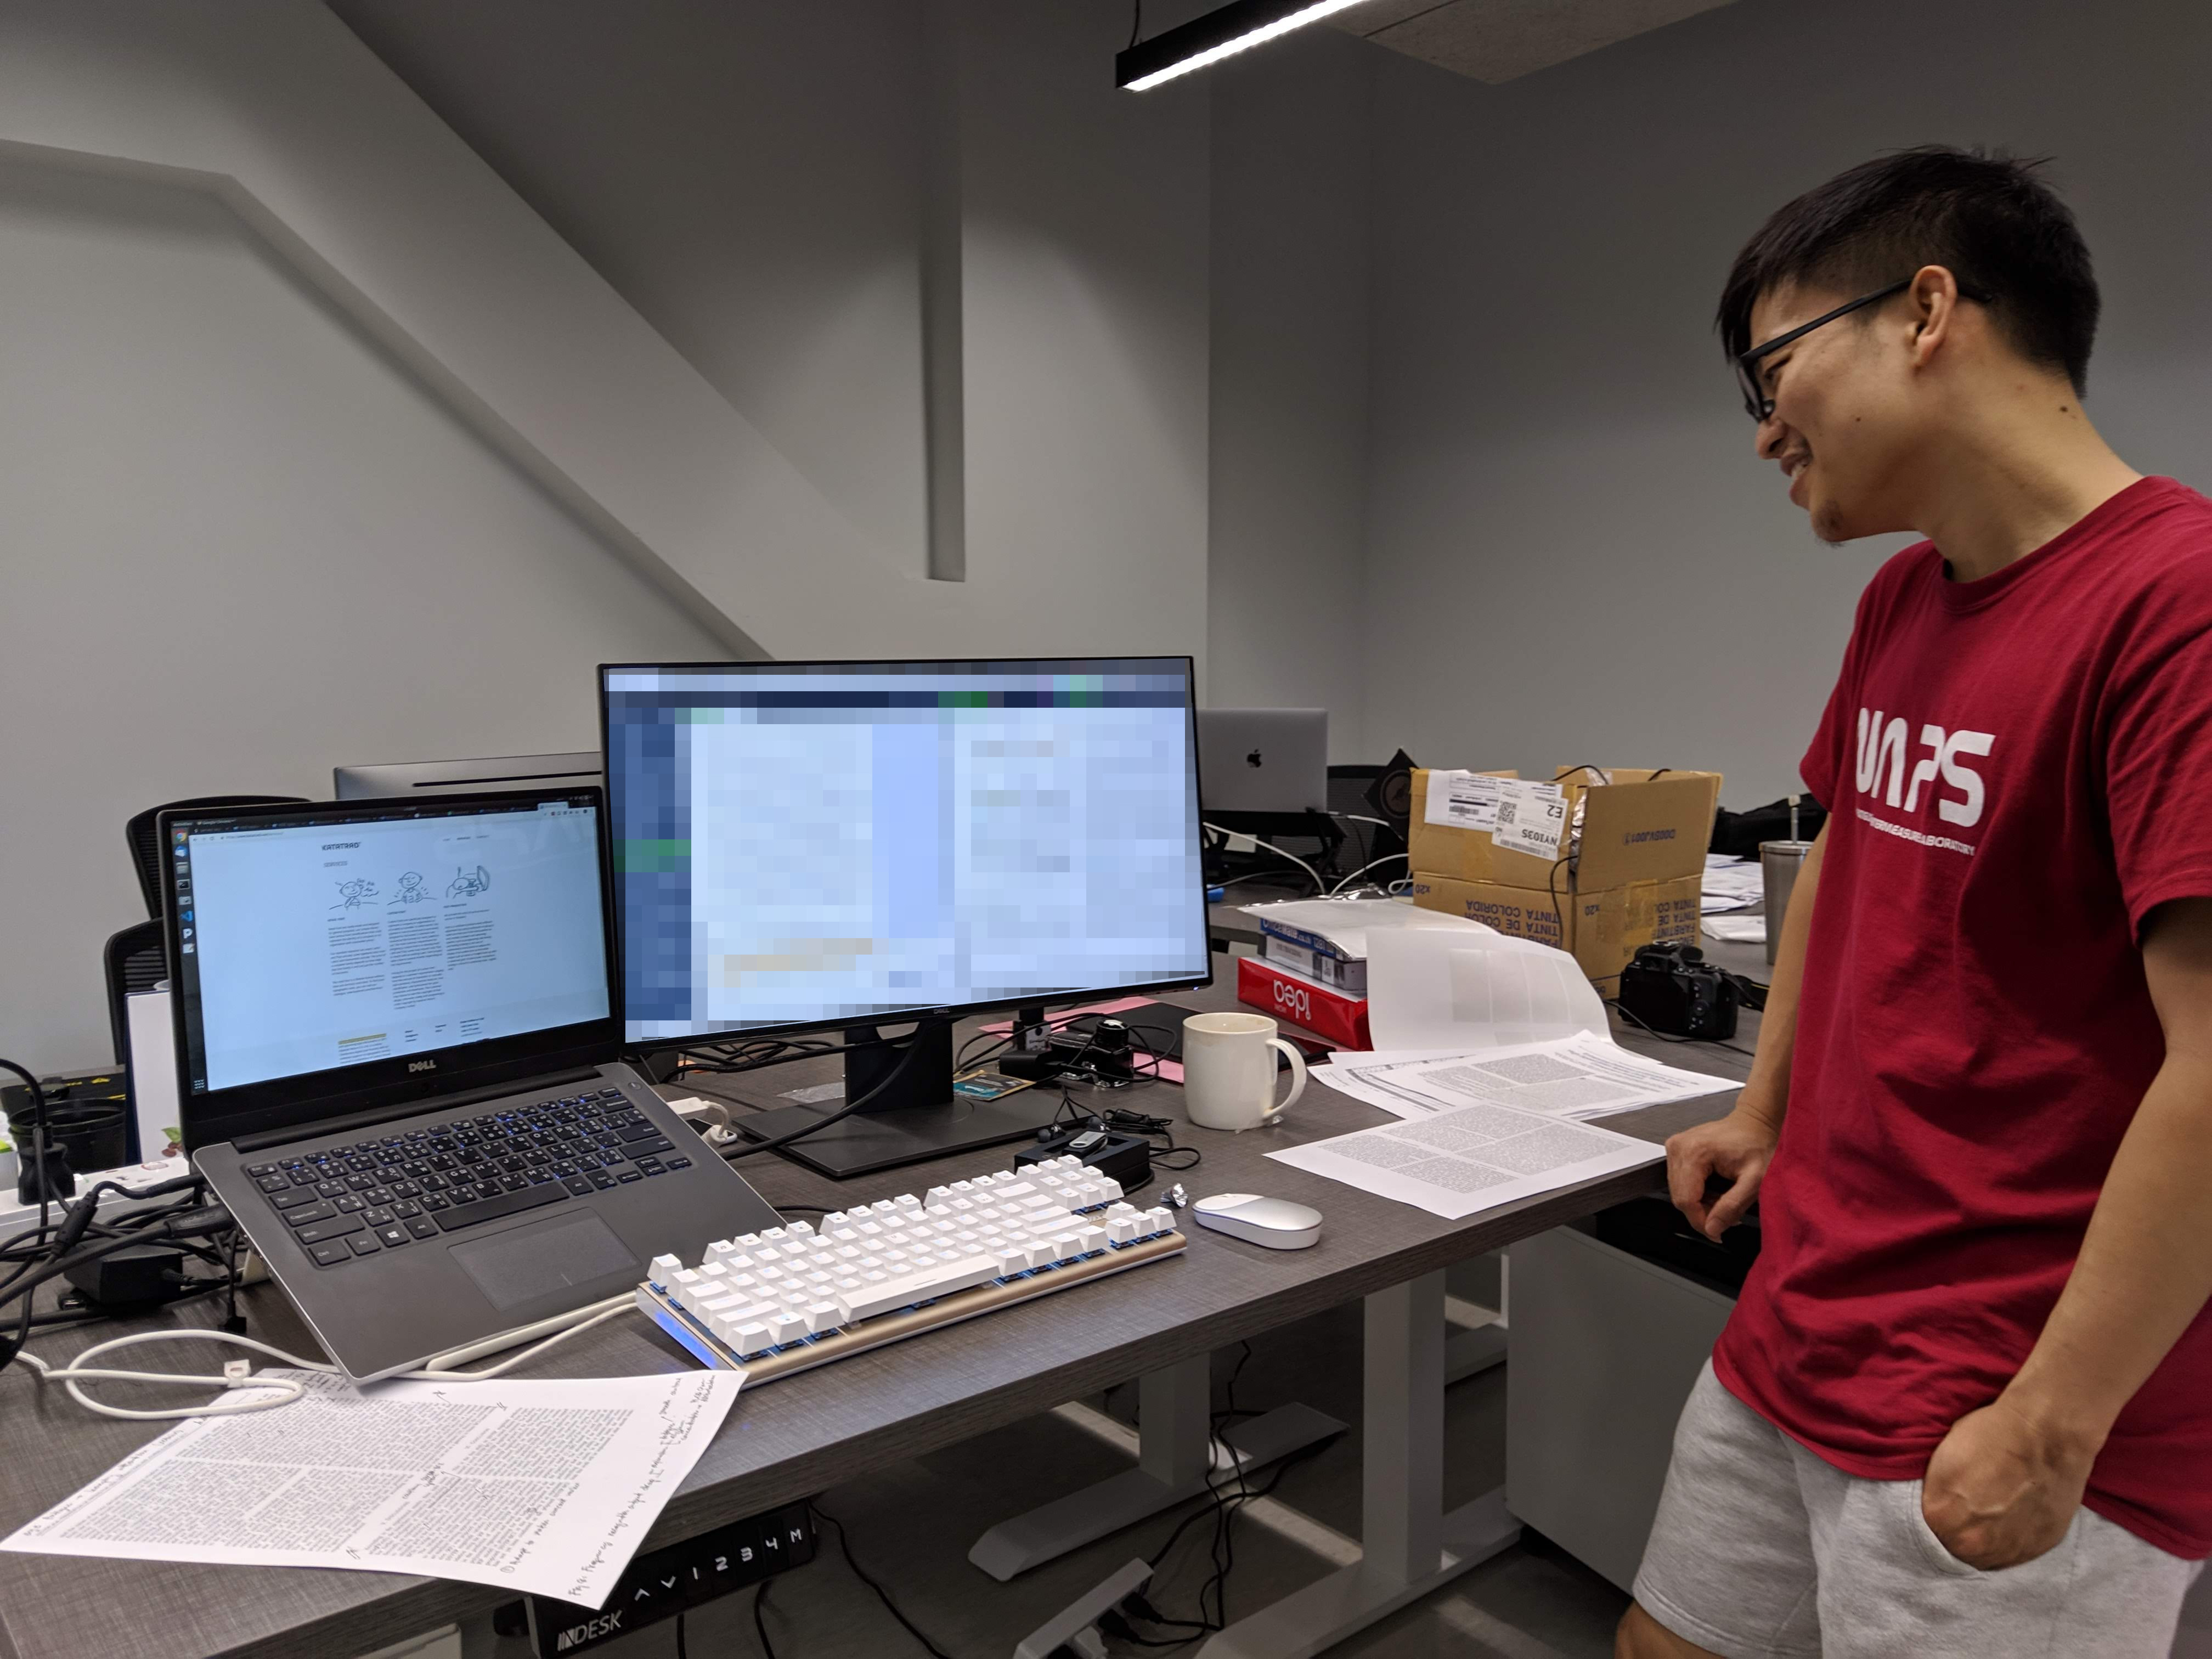
\includegraphics[width=0.55\textwidth]{/home/srakrn/Works/senior/internship/internship_report/diary/images/IMG_20190624_153749.jpg}
    \caption{อาจารย์ธีรวิทย์ วิไลประสิทธิ์พร ขณะทบทวนงานวิจัยโดยคร่าว}
\end{figure}

\section*{ภาพการฝึกงานวันที่ 8/7/2562}
\begin{figure}[H]
    \centering
    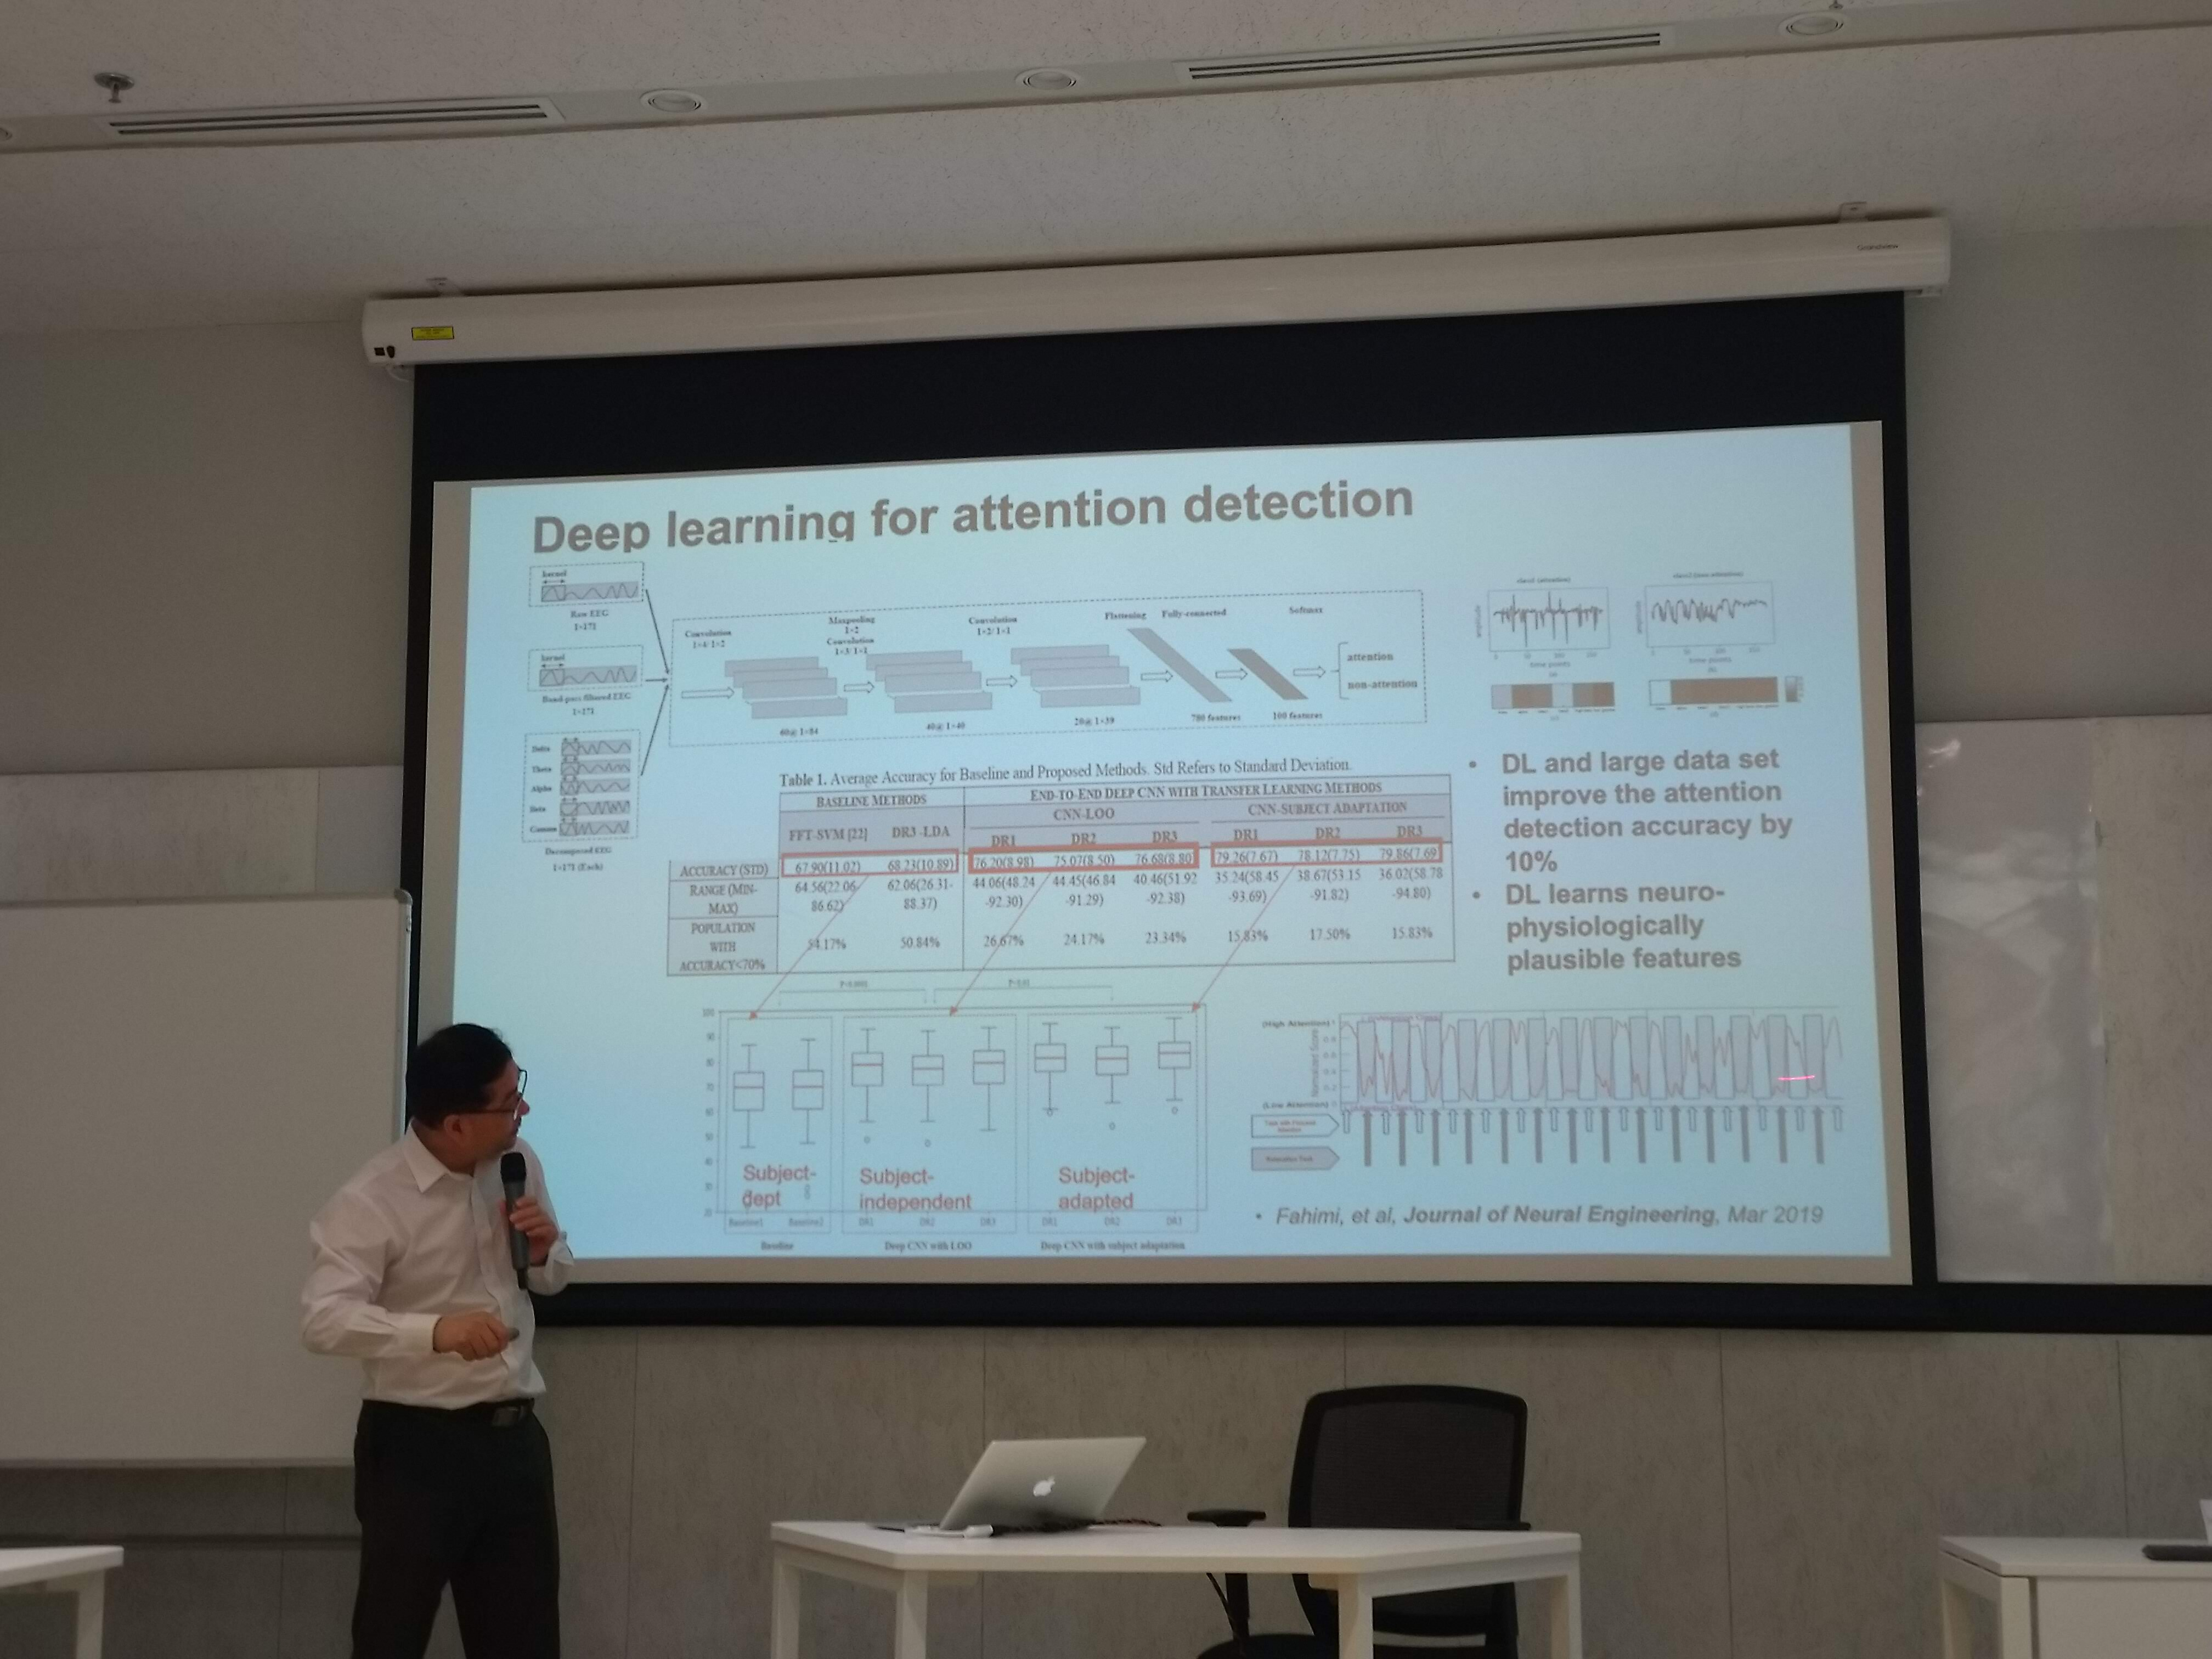
\includegraphics[width=0.55\textwidth]{/home/srakrn/Works/senior/internship/internship_report/diary/images/IMG_20190708_104544.jpg}
    \caption{บรรยายจาก Prof Guan Cuntai}
\end{figure}

\section*{ภาพการฝึกงานวันที่ 23/7/2562}
\begin{figure}[H]
    \centering
    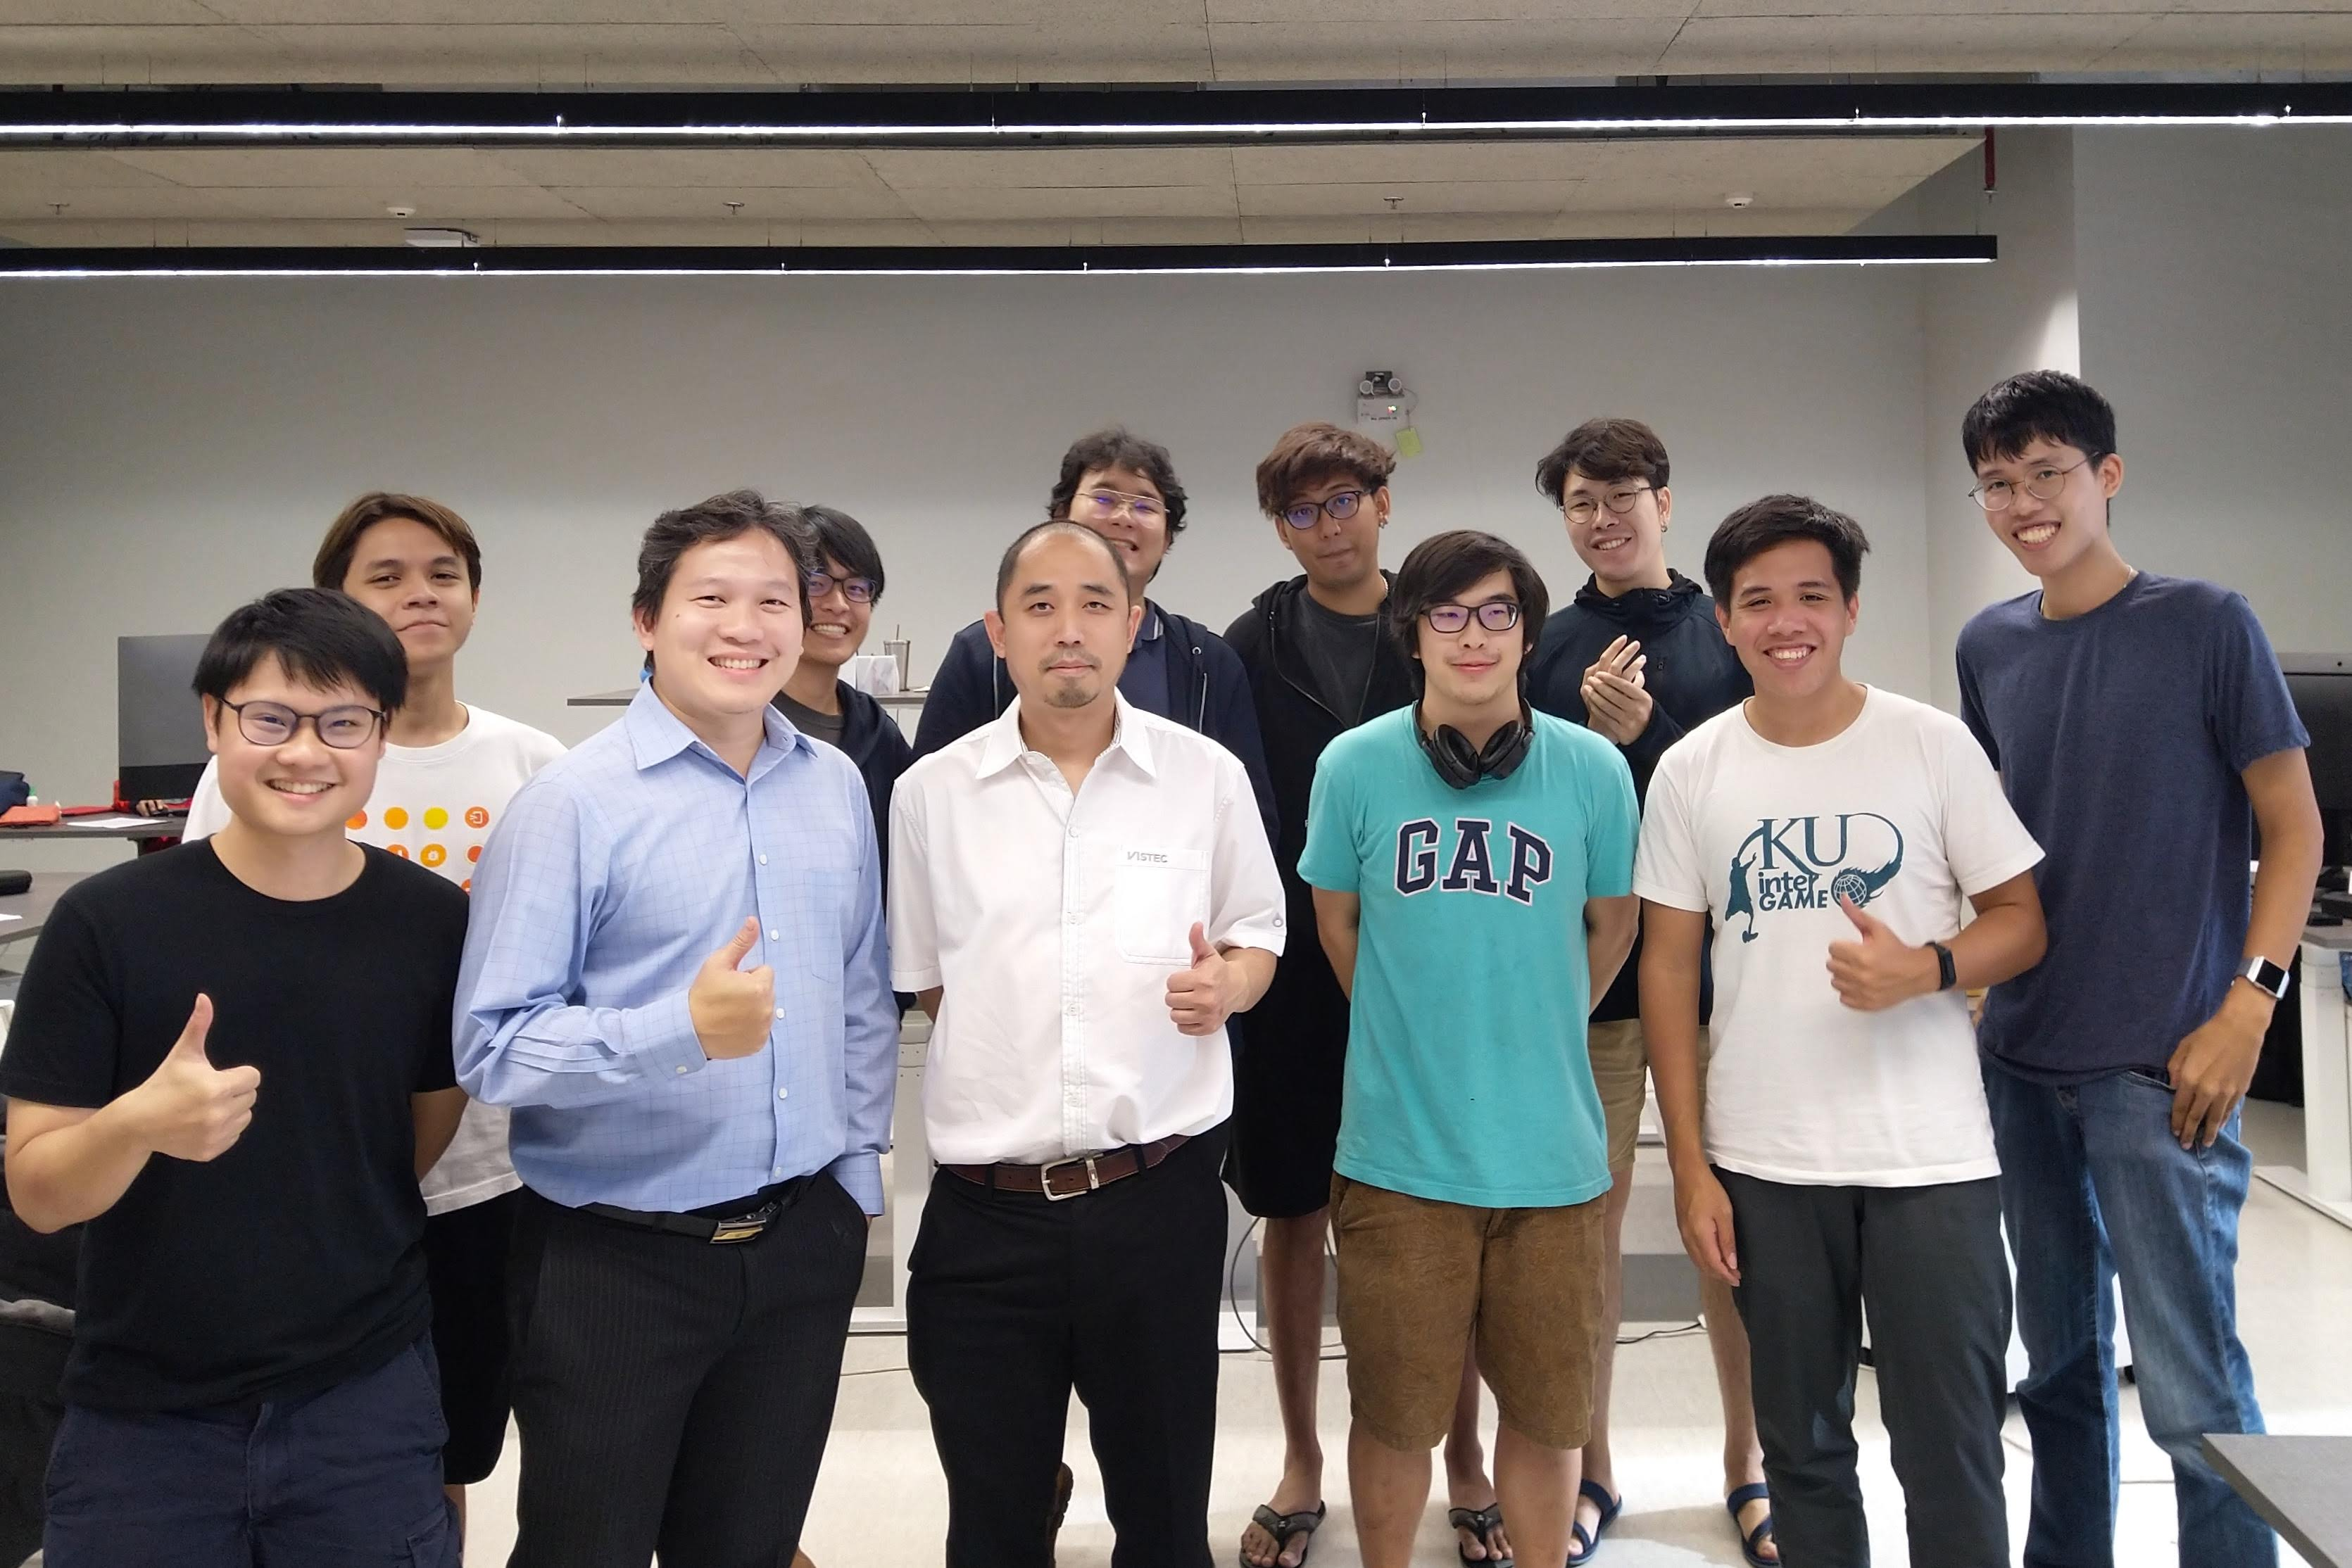
\includegraphics[width=0.55\textwidth]{/home/srakrn/Works/senior/internship/internship_report/diary/images/IMG_20190723_164246-01.jpeg}
    \caption{ทีมวิศวกรรมคอมพิวเตอร์เกษตรศาสตร์ ณ สถาบันวิทยสิริเมธี}
\end{figure}

\end{appendices}
\end{document}